%%%%%%%%%%%%%%%%%%%%%%%%%%%%%%%%%%%%%%%%%%%%%%%%%%%%%%%%%%%%%%%%%%%%%%%%%%%%%%%%
%2345678901234567890123456789012345678901234567890123456789012345678901234567890
%        1         2         3         4         5         6         7         8

\documentclass[letterpaper, 10 pt, conference]{ieeeconf}  % Comment this line out if you need a4paper

%\documentclass[a4paper, 10pt, conference]{ieeeconf}      % Use this line for a4 paper

\IEEEoverridecommandlockouts                              % This command is only needed if 
                                                          % you want to use the \thanks command

\overrideIEEEmargins                                      % Needed to meet printer requirements.

% See the \addtolength command later in the file to balance the column lengths
% on the last page of the document

% The following packages can be found on http:\\www.ctan.org
\usepackage{subfig}
\usepackage{graphicx} % for pdf, bitmapped graphics files
%\usepackage{epsfig} % for postscript graphics files
%\usepackage{mathptmx} % assumes new font selection scheme installed
%\usepackage{times} % assumes new font selection scheme installed
%\usepackage{amsmath} % assumes amsmath package installed
%\usepackage{amssymb}  % assumes amsmath package installed
\usepackage{url}
\usepackage{array}
\usepackage{tabularx}
\usepackage{tabulary}
\usepackage{booktabs}
\usepackage{microtype}
\usepackage{acronym}

\acrodef{ide}[\textsc{ide}]{integrated development environment}
\acrodef{vpl}[\textsc{vpl}]{visual programming language}


\title{\LARGE \bf
Bringing robotics into formal education \\
using the Thymio open source hardware robot
}


\author{Francesco Mondada$^{1}$, Michael Bonani$^{2}$, Fanny Riedo$^{2}$, Manon Briod$^{1}$, \\
L\'ea Pereyre$^{1}$, Philippe R\'etornaz$^{1}$ and St\'ephane Magnenat$^{1}$% <-this % stops a space
\thanks{*This research was supported by the Swiss National Center of Competence in Research ``Robotics'' (Thymio robot development and deployment), by GebertRuf Stiftung (design of accessories), by the Swiss NSF project CRAGP2 151543 ``Robotics in schools,'' and by the EU-FP7 project ASSISIbf, no. 601074 (survey on open hardware).
Many thanks to Luc Bergeron and his team at \'ecal.ch for the industrial design of Thymio; Didier Roy, David Sherman and all the INRIA team for their contributions and diffusion in France; Gordana Gerber for the educational material; all the Mobsya team for the effort in production and sale; and Fabian Hahn for the port of Blockly.}% <-this % stops a space``anyone''
\thanks{$^{1}$Francesco Mondada, Manon Briod, L\'ea Pereyre, Philippe R\'etornaz and St\'ephane Magnenat are with the Laboratoire de Syst\`emes Robotiques,
        Ecole Polytechnique F\'ed\'erale de Lausanne (EPFL), Switzerland.
        {General rule for EPFL emails: \tt\small firstname.lastname@epfl.ch}}%
\thanks{$^{2}$Michael Bonani and Fanny Riedo are with Mobsya Association, Renens, Switzerland.
        {\tt\small michael.bonani@mobsya.org} and {\tt\small fanny.riedo@mobsya.org}}%
}


\begin{document}



\maketitle
\thispagestyle{empty}
\pagestyle{empty}


%%%%%%%%%%%%%%%%%%%%%%%%%%%%%%%%%%%%%%%%%%%%%%%%%%%%%%%%%%%%%%%%%%%%%%%%%%%%%%%%
%%%%%%%%%%%%%%%%%%%%%%%%%%%%%%%%%%%%%%%%%%%%%%%%%%%%%%%%%%%%%%%%%%%%%%%%%%%%%%%%

%\begin{abstract}
%Mobile robots are interesting tools for education because of both the enthusiasm they raise and the multidisciplinary nature of their technology.
%However, because of their price, complexity, bias toward specific groups (boys), and unproved educational value, they are still seldom used in schools and edutainment.
%This paper presents a system-design approach and the resulting Thymio robot that tackle these problems in a holistic way.
%We show how this strategy achieved a low price leading to a high demand and raising the interest of teachers.
%The robot and its development environment are open source and the whole project follows an open distribution and participative model.
%Finally, we show deployment statistics proving that the robot is gender- and age-neutral and preliminary results toward assessing the educational value of robots.
%\end{abstract}


\section{Introduction}

Mobile robots are valuable tools for education because of both the enthusiasm they raise and the multidisciplinary nature of robotic technology.
Mobile robots give access to a wide range of fields, such as complex mechanics, sensors, wireless transmission, mathematics, and computer science, among others.
As mobile robots sense the environment and take actions based on their perception, they seem to display \emph{intentions of their own}~\cite{Mondada2001}.
%This fascinates the users of the robot and creates feelings of accomplishment and power when these users engage in creative activities with the robots.
This impression of intelligence, the permeating presence of robots in science fiction, and their projected use in our society give a sense of touching the future.
%Children can spend hours looking at a robot interacting with its environment and adults can approach robots as a new hobby that replaces radio and electronics kits.
%The emotional potential of mobile robots and their varied technology makes them a potential ideal tool for education.

Despite their potential as educational tools, robots are still not as widespread in schools as they could be. Among the possible reasons, we believe that the following five play a key role:
\begin{enumerate}
\item Although many research projects are developing innovative and interesting educational robots, few reach sufficient maturity to become distributed and accessible to schools. 
\item A versatile robot performing interesting behaviors is a complex piece of technology and therefore expensive. 
%Indeed, for having an educational value and providing an interesting level of interaction, a robot must embed a wide set of sensors and actuators.
%Existing platforms with these features cost several hundred Euros.
This prevents most schools, which have a limited budget for equipment, from acquiring educational robots.
\item Introducing robotic tools into teaching activities requires investment in time and training for the teachers~\cite{CERI2008}.
%In Europe, despite a trend to increase the use of technological tools in the learning process, teachers are still insufficiently trained and are reluctant to introduce these tools in their teaching activity~\cite{CERI2008}.
Therefore, to be accepted by teachers, robots must be both accessible with minimal effort and accompanied by well-prepared educational material shared among colleagues. 
%Moreover, infrastructure should be provided to allow the sharing of educational material among teachers.
\item Robot construction, use, and programming is often perceived as a boyish activity in our Western society~\cite{leonard2009lego,nourbakhsh2009robot}.
% For instance, several authors report that girls have such a perception of the LEGO Minstorms~\cite{leonard2009lego,nourbakhsh2009robot}.
This strongly limits the potential of robots as general-purpose educational tools, especially in schools.
\item Finally, many teachers are reluctant to follow volatile trends, especially if these are based on purely commercial arguments.
Teachers prefer to invest in stable tools, in contrast to trends in current consumer technology. %, which is often very volatile and based on continuous renewal rather than on durability.
\end{enumerate}

Open source hardware projects can address several of these issues in a different way than closed-source purely commercial products. 
By \textit{open source hardware} we mean, following the definition of the Open Source Hardware Association,\footnote{\url{http://www.oshwa.org/definition/}} ``hardware whose design is made publicly available so that anyone can study, modify, distribute, make, and sell the design or hardware based on that design.''
In this paper, we show that this concept, implemented in the Thymio project through a community of users, developers and manufacturers, brings a strong added value to the robot and to the educational methods.
In addition, we compare our experience with other robotics open source hardware projects not focused on education and highlight challenges and opportunities specific to education.

\section{Related Work}

Many publications present educational robots, from low-cost systems targeting Africa~\cite{Rubenstein2015,Gyebi2015} to extremely sophisticated humanoids~\cite{Hood2015,Mazzoni2016}. 
Among those, only a handful are commercially available, limiting their validation by educational scientists, who are typically not roboticists.
As a result, 90\% of publications about validation of educational results have been based on LEGO\textsuperscript{\textregistered} Mindstorms\textsuperscript{\textregistered}~\cite{benitti2012exploring}, a widely available commercial product.
The latest version, EV3\footnote{\url{http://mindstorms.lego.com}}, is expensive ($\approx$ US\$400) but offers a wide range of possibilities, especially at the mechanical level using LEGO\textsuperscript{\textregistered} bricks and at the software level with its graphical programming environment. 
%NOTE: SM: commented WeDo to save space and streamline story
%At a lower price, LEGO\textsuperscript{\textregistered} proposes the WeDo\textsuperscript{\textregistered} system ($\approx$ 80\,\$).
%The WeDo\textsuperscript{\textregistered} is similar to EV3 but only reads one sensor and controls one actuator and must always be connected to a desktop computer.
%In comparison, the BeeBot robot\footnote{\url{http://www.beebot.org.uk}} is a cheap ($\approx$ 90\,\$) mobile system.
%However, it is not a real robot but rather an automaton: There is no perception of the environment, just a good encoder for precise movements and a simple programming interface based on buttons giving directions for the movement.
Among the other players on the market is the Edison robot\footnote{\url{https://meetedison.com/}}, which is extremely low cost (US\$49) and compatible with LEGO\textsuperscript{\textregistered} bricks. 
The low price has pushed drastic design choices: small size, weak motors, few sensors, communication with the computer by audio jack and standard AAA batteries not included in the price.
These choices strongly limit its possible usage.
%Among widely used robots, none is part of an open source hardware project.

Among the robots available on the market, only a few are open source and are used in schools:
Scribbler2, produced and sold by Parallax\footnote{\url{http://www.parallax.com}} ($\approx$ US\$180), is a 188\,mm large robot, designed to run on the ground and equipped with a few light sensors, one distance sensor, two ground sensors, and few \textsc{led} displays.
It runs on standard AA batteries and has a hacker port for interfacing electronic extensions.
It is programmable with a graphical or a textual code interface.  
The main weakness of Scribbler2 is its limited number of sensors and compatibility with other systems. 
Moreover, there seems to be no active community around its development.
The e-puck~\cite{mondada2009puck} robot targets university-level education.
Well equipped with sensors and actuators, modular and compact, it can be programmed with industry-standard environments.
Several simulators allow running highly complex experiments. 
%There is an active community of users and developers around it.
Its main weakness is its high price ($\approx$ US\$870).
Finch\footnote{\url{http://www.finchrobot.com/}} ($\approx$ US\$99) is a very simple robot that has been designed around a wired connection to the computer. 
This connection reduces electronics requirements, such as batteries or wireless communication, and allows control to be implemented entirely on the computer.
This results in availability of a very broad set of possible programming languages, which is the real force of this robot. 
However, the cable does not allow real autonomy and mobility.
Finally, the mBot\footnote{\url{http://www.makeblock.cc/mbot/}} is a mobile platform based on an Arduino board.
Its electronics is simple and inexpensive and the robot only features a couple of sensors, which allows drastic reduction in its price ($\approx$~US\$75), but also limits the perception possibilities and therefore the span of use.

With respect to these robots, Thymio has a compact size (110\,mm), many interaction possibilities, an affordable price (US\$130), and a large set of sensors.
%Its design makes the best use of the recent cheap components coming from the explosive growth of the mobile devices market. 
To the best of our knowledge, beside Thymio there are no educational products providing a similar integration of sensors and actuators at a lower price.

Teachers, from primary school up to high school, are a primary target user group of the Thymio project.
They decide which tools are used in their class and are key people in the education ecosystem.
For teachers, the motivation to use robotic tools depends on many factors~\cite{chevalier2016}.
Among them, the availability of materials and training plays a key role.
%The BeeBot mentioned previously, because of its radical simplicity, is one of the tools that needs the least training. 
%Moreover its use in learning activities is based on a simple grid on a printed map on the ground, allowing fast and easy integration in existing lessons.
%These are probably two important factors for its success in schools~\cite{2008highfield,2008demichele} and the availability of a rich set of educational material\footnote{\url{https://www.learningplace.com.au/deliver/content.asp?pid=38840} and \\ \url{http://beebots.skola.edu.mt/}}.
%However, the total lack of sensors reduces the BeeBot to an automaton, easy to use but limited to activities implementable by sequences of motions, without any closed-loop control that would allow teaching computational thinking or robotics concepts.
The development of educational material and courses to train teachers requires a huge effort, based on a good mix between robotics and educational skills. 
Moreover, educational material varies from school to school, as requirements are very dependent on local educational programs and languages. 
%For example, in Switzerland, every of the 26 states composing the country has its own school program and its own language among the four national ones. 
%Educational material and the related training must therefore be adapted to each situation.
Even for large companies like LEGO\textsuperscript{\textregistered}, such a development is not sustainable. 
A crowd-sourcing approach may solve this problem; An active community of users can contribute to the development of the material in a distributed manner, adapting the material to the local situation.
LEGO\textsuperscript{\textregistered} itself is moving this direction by promoting communities of users~\cite{Hienerth2014} with a user-producer interaction similar to that of open hardware projects.
An open source community regrouping developers, manufacturers, and end users is therefore a very interesting model to address the distributed development and sharing of educational material and the diffusion of training sessions.
%This model is an extension to education of what is already practiced in projects such as Arduino~\cite{Jamieson2010}.
In this paper, we study a case of implementation of this model.

%Several initiatives have focused on increasing the rate of females in engineering in general and in robotics in particular~\cite{weinberg2007impact}.
%Roberta~\cite{2010bredenfeld} is one of the largest and uses the LEGO Minstorms.
%Recent work has shown that a different approach to robotics, for instance linking with arts and proposing creative workshops~\cite{nourbakhsh2009robot}, can improve the attractiveness for girls. 
%Some researchers have created hardware tailored to crafting activities, such as the PicoCricket~\cite{2008rusk} which is close to the NXT but does not require LEGO construction.
%Compared to these works, Thymio aims at being attractive for both genders.

%Several studies have measured the impact of the use of robots on children~\cite{weinberg2007impact,nourbakhsh2009robot,sinkele2010effectiveness}, but none of these provide quantitative data on the usage of the different features of the robot.
%On the contrary, Thymio can log the usage of its features, providing a tool to monitor the progress of children and to investigate the value of different curricula.


\section{Design choices}

\begin{figure}
   \centering
	\includegraphics[width=.8\columnwidth]{figures/front_2016}
	\vskip 1.0em
	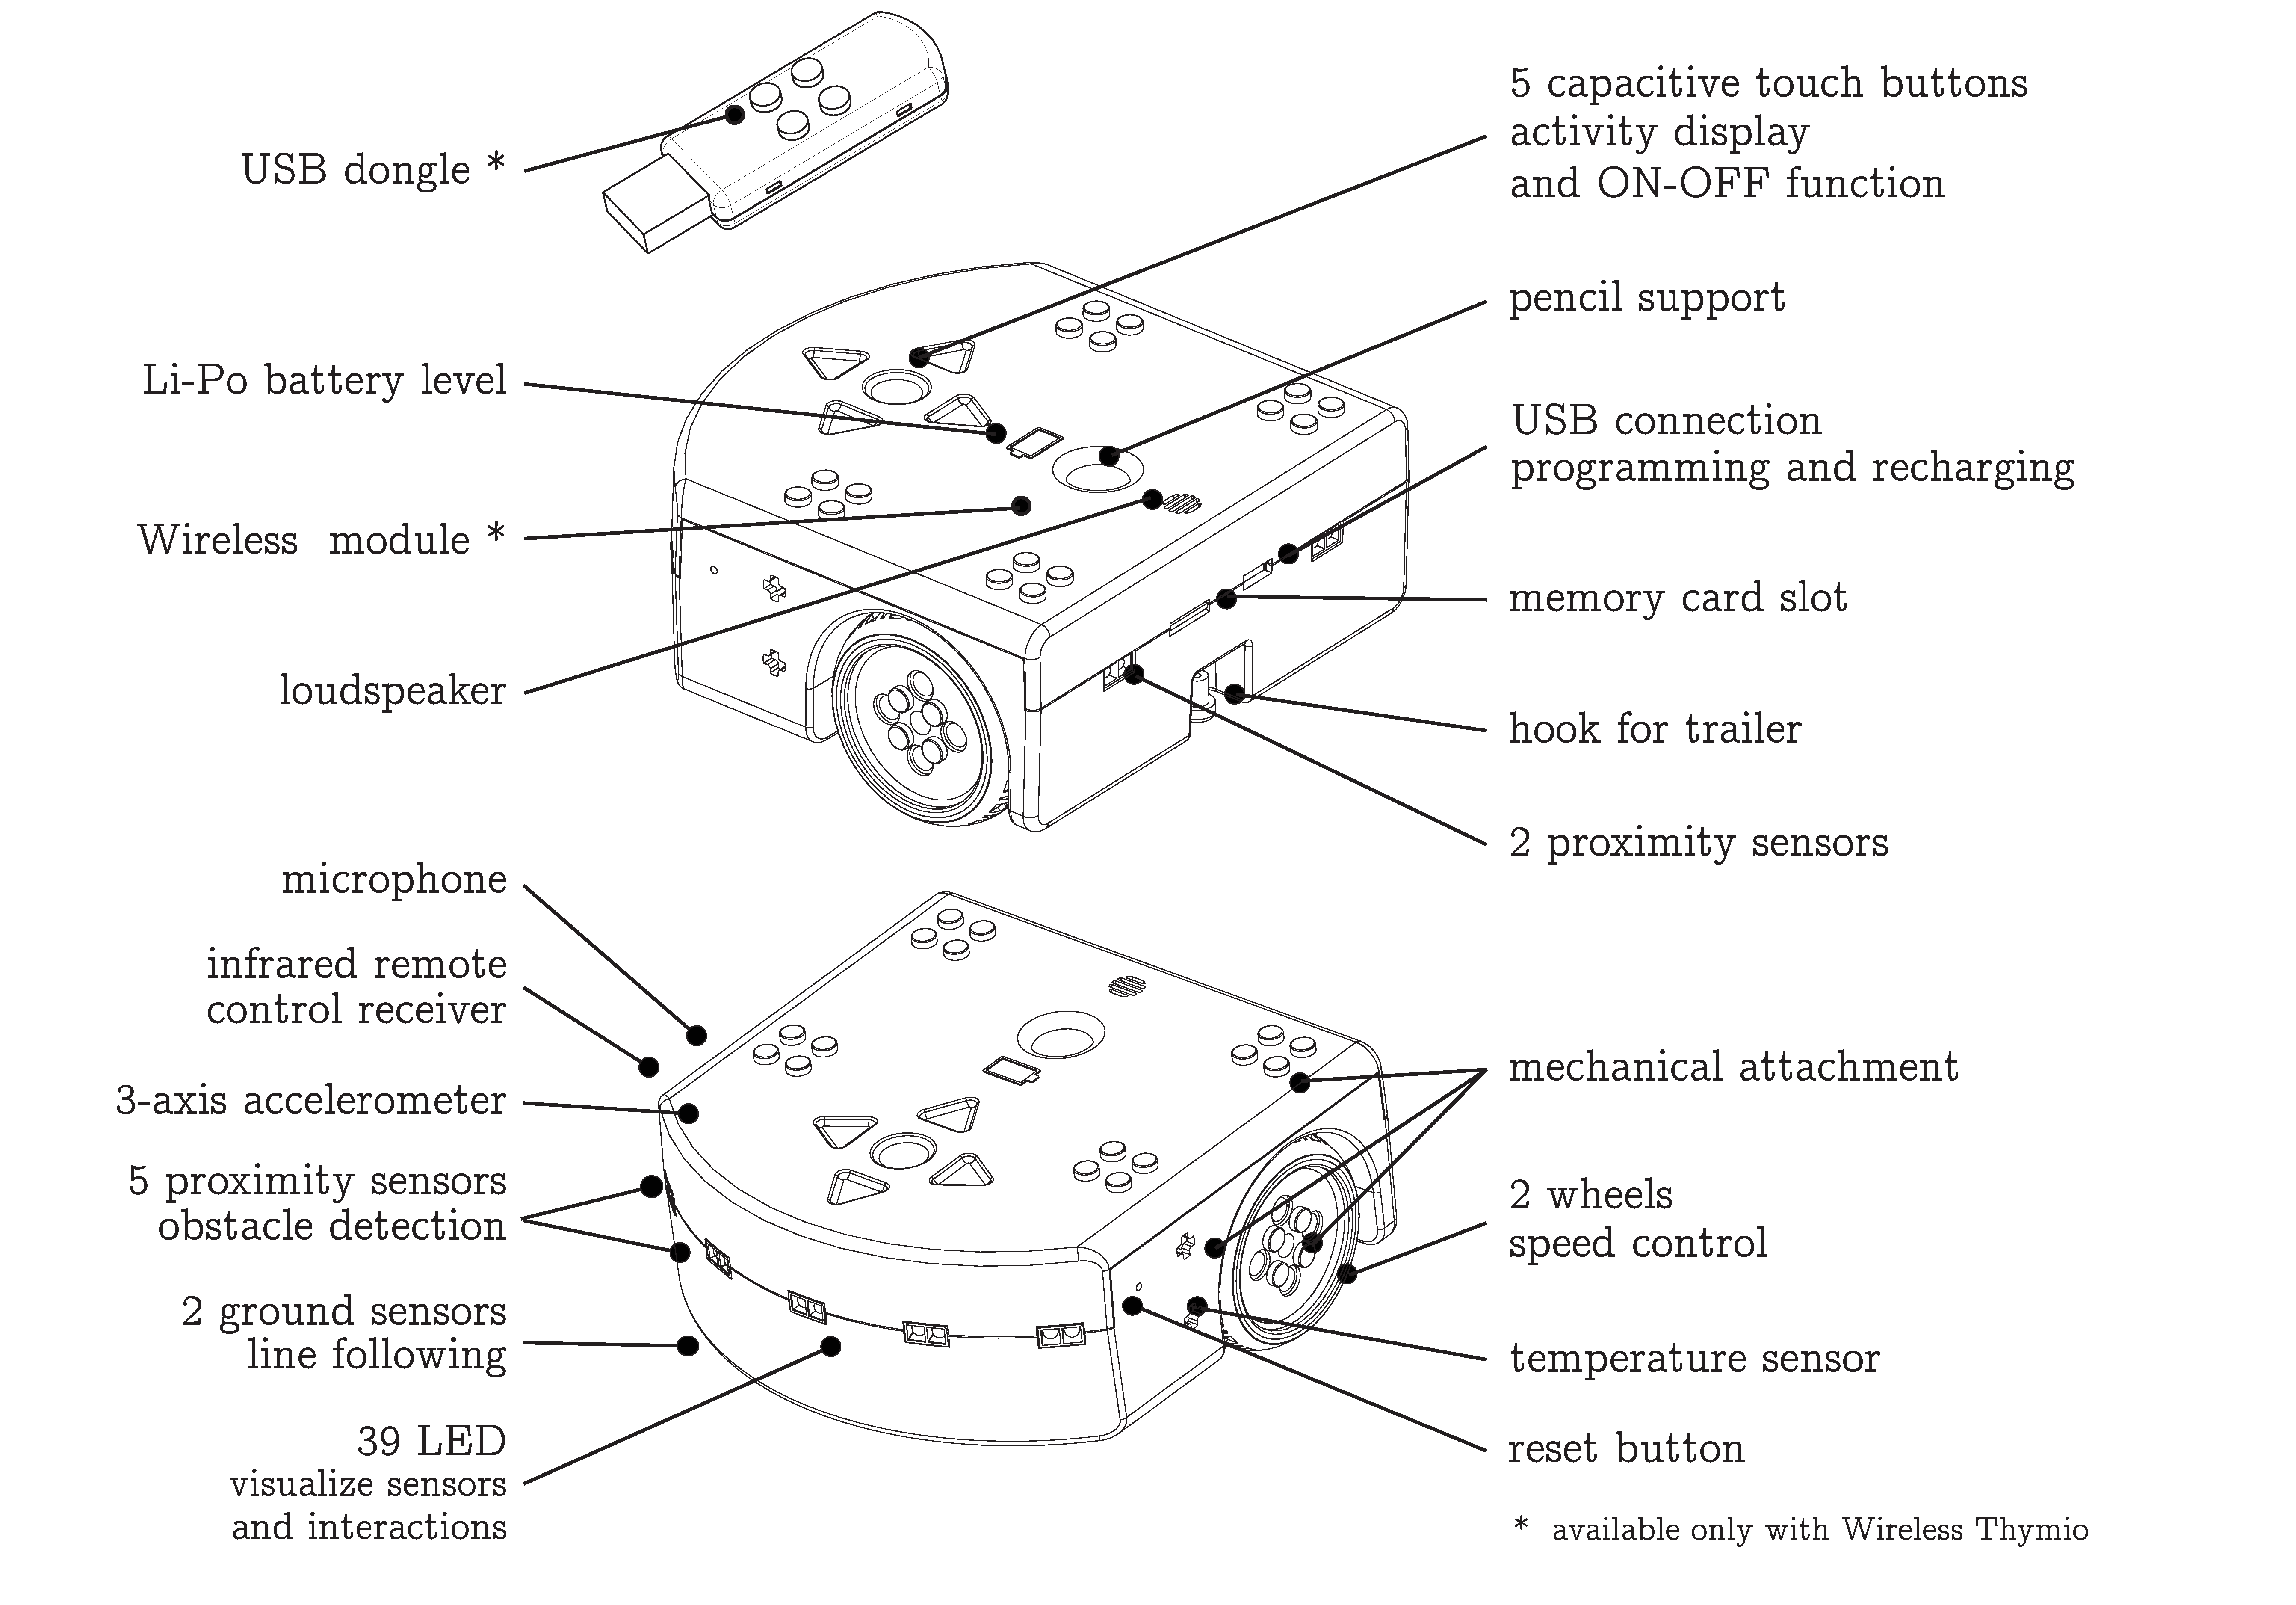
\includegraphics[width=\columnwidth]{figures/wirelessThymioVecto}
	\caption{The Thymio robot and its main components for the wireless- and the \textsc{usb}-connected versions.}
	\label{fig:schematique}
\end{figure}


We designed the Thymio robot along seven main axes: a low price to address a larger number of users; a feature set that suits both genders and multiple ages from young children to adults; a mechanical design that promotes creativity; a combination of sensors, actuators, and programming features that facilitates learning: a set of ready-to-use programs to quickly access robotic behaviors; an accessible programming environment; and an open source community contributing to design and dissemination.
The result is a miniature differential-wheeled robot suited for use on a desktop (Fig.~\ref{fig:schematique}, top).
The robot is robust enough to be mishandled by children; it can fall from a table without breaking.
It features a translucent white hull and a wide range of sensors and actuators (Fig.~\ref{fig:schematique}, bottom).
The robot has an embedded battery, rechargeable by \textsc{usb}, that provides 3 to 5 hours of power.
More details on the robot and the previous research results can be found in~\cite{RiedoPhD, magnenat2014}.  

\subsection{Low Price}

Price is key in the adoption of robots by schools~\cite{kradolfer2014sociological}.
Thus, the design of Thymio targeted low production costs while including a broad range of functionalities enabling flexibility.
%Therefore the design of Thymio had to target a low production cost, while including a broad range of functionalities to enable flexibility in its use. 
As in this type of robot the main cost comes from electronics and sensors~\cite{thesis_michael}, we focused on low-cost sensors that allow rich interactions with both the environment and the user.

The resulting Thymio robot possesses a large number of simple sensors:
seven horizontal proximity sensors, two ground sensors, a three-axis accelerometer, a thermistor, and a microphone.
Five capacitive touch buttons organized as a direction pad form an intuitive user interface.
Compared to physical buttons, these simplify the plastic hull of the robot and make it more robust.
A remote control receiver provides additional distant buttons.
%A microphone can record sounds and detect claps. 
%Finally, a thermistor measures temperature.
Most of these devices cost less then US\$0.20, the most expensive being the accelerometer with a cost of about US\$0.80, which is an acceptable price given the possibilities it brings to the robot.
%The omnipresence of this type of sensors in smartphones and compact cameras has drastically lowered their prices over the last decade.
We also chose low-cost toy motors and control them in speed (max. 13\,cm/s) measuring the back-electromotive force and therefore removing the need for additional encoders.

%However, choosing the optimal combination of sensors and processor is a difficult problem, as hardware interfaces are limited on a microcontroller and therefore compromises must be made.
We evaluated several microcontrollers and chose the PIC24F from Microchip because it integrates a \textsc{usb} interface and can drive capacitive touch buttons directly, saving additional components. 
This microcontroller controls all sensors and actuators, with the exception of the internal Li-Po battery recharging logic, which uses a specific chip for safety reasons.
%This choice of a single microcontroller led us to non-trivial design decisions like using low-cost shift registers to drive the many \textsc{led}s.
%Moreover, instead of directly connecting the infrared sensors to an analogical input, we interface them using a comparator that transforms the analogical signal into a binary one with a pulse having a duration proportional to the intensity of the original signal~\cite{wanda}. 
%This design saves \textsc{cpu}-time, reduces power consumption (it allows a shorter infrared pulse than with an analogical design) and allows to use the sensor for communication.  

For our specific design, we needed custom-made mechanical parts.
To reduce the price, all mechanical parts are injected plastic, for a total production cost of less than US\$4.

Our choice of electronic components implies production that is either fully automatized or includes some manual operations. 
Full assembly is required in order for the robots to be certified for use by children. 
%A final assembly by the user is excluded by the certification required in the case of use by children. 
As a full automatization requires investments that are beyond the possibilities of this project, the current production is based on some manual operations. 
We therefore decided to produce in China, where manual work is less expensive.
%This is a very critical choice in open source hardware projects, and we will discuss this issue in detail in the next section.
We have thus far produced more than 15,000 robots in batches of 1,000 units, with a cost per robot of US\$35.
%Because manual work is expensive in western countries, we produce through subcontractors in China.
%Indeed, while most of the electronics consists of \textsc{smd} components mounted by a robot, some are soldered (sensors, microphone, \textsc{led}s) by hand and the robot is also assembled by hand.
%We streamlined the production of plastic parts (Thymio has only 5 parts while our previous prototype had 11) and opted for injection molding. 
%The plastic hull consists of two main parts screwed together to facilitate the vertical assembly and disassembly of the robot.
%Moreover, when selecting features we took into consideration the complexity of the injection mold.
%The design of the mechanical parts has been aligned with these choicesthat are injected, resulting in all custom parts of Thymio costing less than 4\,\$.
%In these conditions Thymio costs 35\,\$. 
The strict quality control, the production management, the support to the users, and the margins for distributors result in a final selling price of US\$130.

\iffalse
\begin{table}
\centering
\begin{tabularx}{\columnwidth}{ll}
\toprule
Description & Price (USD)\\
\midrule
electronic components & 15\,\$ \\
microcontroller & 4 \$ \\
motors & 2 \$ \\
plastic parts (hull, wheels, and light guides) & 4 \$ \\
assembling & 8 \$ \\
transport & 2 \$ \\
\bottomrule
Total & 35 \$ \\
\end{tabularx}
\caption{Production cost of \textsc{usb}-connected Thymio.}
\label{tbl:thymio-price}
\end{table}
\fi

%Thymio finally costs 35\,\$ per unit when produced in a batch of 1\,k units, with fixed fees of 15\,k\$ (13\,k\$ for the mold and 2\,k\$ for the \textsc{ce} certification).
%This allows a selling price of \textsc{chf}\,129 ($\approx$ 130\,\$).

\subsection{Multi-Age and Gender-Neutral Feature Set}
\label{sec:multi}

Several design choices, like the variety of sensors, the multiple ways of interacting with the robot, the neutral hull design, the various programming environments, and the possible customization with accessories, contribute to make Thymio accessible to girls and boys of different age groups from kindergarten to university~\cite{Riedo2013}.
These design choices were made and implemented thanks to an important contribution by industrial designers of the University of Art and Design of Lausanne.\footnote{\url{http://www.ecal.ch}}
The white neutral hull is a key element in this set of choices, and it is the opposite of the technical look chosen for the Edison or the LEGO\textsuperscript{\textregistered} robots. 
These latter two robots implicitly target a group of people interested in technical systems, mostly males, while Thymio is open to both genders and a larger target audience.
%The white hull is initially neutral and children can choose their own color using the \textsc{rgb} \textsc{led}s or attach accessories to the hull.

\iffalse
This impacts also on the type of activities:
The youngest play with the robot through a set of basic behaviors (see section \ref{sec:behaviors}) and can use Thymio as a support for handicrafts or construction.
%and the older can program it (see section \ref{sec:aseba}).
%The different basic behaviors are selectable using the capacitive buttons and show some of the capabilities of the robot, such as obstacle avoidance, slope climbing, etc.
%By interacting with the different behaviors, for instance by blocking the robot with the hand and seeing it avoiding it, children can discover the concept of the sensory-motor loop. 
%As every behavior has a different color, children can also understand that different \emph{programs} run on the robot.
%Children around 6 can use Thymio as a support for handicrafts or construction.
%For example, they can create kinetic sculptures.
For children above 9 years old and adults, Thymio is suited to introduce programming and robotics.
Learners can start by programming new interactive behaviors (see section \ref{sec:aseba}) and can go on with constructing around the robot and programming a behavior that interplays with the construction.
High school and university students can use the robot to learn advanced robotics concepts through the integration with \textsc{ros}~\cite{quigley2009ros}.
Teachers can use this flexibility of use to adapt the look and the behavior of Thymio to their teaching activities, or even introduce this adaptation as activity in handicraft or computer science lessons.
Moreover users looking for additional hardware features can interface Thymio with other open hardware devices, such as computer boards\footnote{Interface with a Raspberry PI under \url{https://www.thymio.org/en:thymioexplorer}} or other robotic mechanics\footnote{Interaction with the Poppy open source hardware under \url{https://youtu.be/0otXtF8J_Z4}}.
Finally, because of the open-source and open-hardware nature of the project, advanced programmers can improve their skills in C by modifying the firmware or in electronics by disassembling the robot.
\fi

\subsection{Promoting Creativity}
\label{sec:crea}

%We wanted the robot to be a starting point for users to invent their own creations.
%Therefore, we thought Thymio as a support for handicrafts and constructions.
The white neutral hull is also meant to represent a blank page that can be decorated and drawn upon, and the hull's shape allows easy integration into a larger structure.
%The robot features a hole in its middle to insert a marker for drawing.
%It also has a slot for a microSD card, allowing users to add their own sounds or to load a pre-compiled code by the simple insertion of a dedicated card.
The square format of the hull facilitates the use of the robot as a base for the user's own constructions.
To that end, Thymio is compatible with LEGO\textsuperscript{\textregistered} bricks, both on the body than on the wheels. 
This last connection can be used to actuate elements elsewhere in the added structure (Fig.~\ref{fig:example-construction}, third row left) or to lift the robot's own weight (Fig.~\ref{fig:example-construction}, third row right).
%There are four attachment positions on the top of the robot and two LEGO\textsuperscript{\textregistered} Technics crosses on each side.
%Additionally, the two wheels have attachment points, which permits to use them to actuate elements elsewhere in the structure (Fig.~\ref{fig:example-construction}, third row left) or to lift the robot's own weight (Fig.~\ref{fig:example-construction}, third row right).
Therefore, we chose more powerful motors than strictly necessary to move the robot around.
%The same fixation points used for LEGO\textsuperscript{\textregistered} bricks can be used to attach paper structures.
Paper can also be used to change the body shape or add body movements, as illustrated in Fig.~\ref{fig:example-construction} by the orca, opening and closing its mouth while moving forward, or by the bat, moving its wings. 
But paper and cardboard can also radically change the locomotion principle, as illustrated in the second row of Fig.~\ref{fig:example-construction} by the zombie, where the wheels of the robot activate the legs. 
The paper structure can also be used to interact with the sensors, as illustrated in the second row of Fig.~\ref{fig:example-construction} by the bear, which extends its paw in front of the sensors to drive its iceberg (the robot).
The same fixation points can be used to attach 3D printed customized parts, as illustrated by the winder shown in the fourth row of Fig.~\ref{fig:example-construction}.
Moreover, one can use paper to create environments, either flat with patterns that can be used in association with the ground sensors (Fig.~\ref{fig:example-construction}, bottom) or 3D objects, such as the trees beside the zombie in Fig.~\ref{fig:example-construction}.
Finally, it is also possible to link several Thymio by software, allowing the coordination of complex multi-Thymio robotic structures.

\begin{figure}
\includegraphics[width=.49\columnwidth]{figures/orca}\hfill\includegraphics[width=.49\columnwidth]{figures/bat}
\vskip .5em
\includegraphics[width=.49\columnwidth]{figures/zombie}\hfill\includegraphics[width=.49\columnwidth]{figures/ours}
\vskip .5em
\includegraphics[width=.49\columnwidth]{figures/moving-heli}\hfill\includegraphics[width=.49\columnwidth]{figures/funi}
\vskip .5em
\includegraphics[width=.49\columnwidth]{figures/both_half_winder}\hfill\includegraphics[width=.49\columnwidth]{figures/winder_on_thymio2}
\vskip .5em
\includegraphics[width=\columnwidth]{figures/5senses}
\caption{Examples of extensions of the Thymio basic robot with paper or cardboard body extensions (top four images), using LEGO\textsuperscript{\textregistered} structural extensions (third row), using 3D-printed extensions (fourth row) or using a printed environment (bottom).}
\label{fig:example-construction}
\end{figure}



\subsection{Facilitating Learning}

When designing Thymio, we took care to provide many incentives for the users to learn new things throughout their direct interaction with the robot.
This translates into specific hardware and software choices.

At the hardware level, we render visible the activity of the various robot components by adding an \textsc{led} next to each of them, for a total of 39 \textsc{led}s.
These \textsc{led}s locally color the hull and allow the user to see immediately where and when the robot perceives a change in its environment: proximity of objects, changes in the ground color, temperature, sound, or accelerations.
%\textsc{led}s show, by their light intesity or their color, the measurements of the proximity sensors, the temperature sensor, the microphone, and the accelerometer. 
Some \textsc{led}s display data exchanges from the infrared remote control receiver or with the microSD card. 
The capacitive buttons give both visual and acoustic feedback.
%There is a \textsc{led} next to each proximity sensor that lights up as soon as an object is close enough to be seen, and shines brighter the closer the object gets.
%Similarly, a combination of blue and red \textsc{led}s show the temperature, and the infrared remote control receiver and the microphone both have \textsc{led}s that flash when they detect something.
%On the top of the robot, a circle of 8 \textsc{led}s shows the 3D inclination of the robot thanks to the accelerometer. 
%This circle is also used to reflect some of the behaviors of Thymio.
%Finally, two strong \textsc{rgb} \textsc{led}s color the whole top of the robot.
%In addition to a visual feedback, the capacitive buttons also have an acoustic feedback.
The link between a sensor and its feedback can be turned off when programming the robot so that the \textsc{led}s and loudspeaker can be used for other purposes.

At the software level, we provide a set of programming environments (see the Programming Environment section below) that enable beginners to discover programming progressively.
First, we teach them the basic rules of programming using a purely visual interface, then they discover the construction of syntax trees by assembling graphical blocks, and finally we provide a full text-based coding environment with advanced debugging tools, such as real-time inspection of the variables of the robot and plotting features, providing a visual way to understand time-related concepts.
%Robotics experts can program Thymio using the \textsc{ros}\footnote{accessible through the \emph{asebaros} bridge, see \url{http://www.ros.org/wiki/asebaros}} environment~\cite{quigley2009ros}.


\subsection{Fast Access to Robotics Behaviors}
\label{sec:behaviors}

Many existing robots need to be built or configured before showing any operational behavior. 
For instance, the Edison robot needs to read a bar code and the mBot needs to be assembled.
This can be a barrier for school activities, one we wanted to avoid; rather, we wanted a robot able to show interesting behaviors right out of the box.
Therefore, Thymio has six different basic behaviors, stored in flash permanently, accessible as soon as the robot is started.
These basic behaviors allow people starting Thymio to immediately interact with it, while illustrating the many possibilities of the robot.
%The behaviors are interactive.
%For each behavior, the robot's body has a different color, allowing the user to easily recognize it.
%The user can navigate between the colors with the buttons and select the behavior she/he wants to use.
%These behaviors can be exploited in a construction to create reactivity without the use of programming, such as in the paper creations shown in the top four images of Fig.~\ref{fig:example-construction}.
The user can begin creating constructions on top of these basic behaviors without the need for programming, such as in the paper creations shown in the top four images of Fig.~\ref{fig:example-construction}.

\iffalse
\begin{table}
\begin{tabularx}{\columnwidth}{@{}llll@{}}
\toprule
mode & color & sensors & behavior \\
\midrule
friendly & green & infrared (IR) & follows an object at distance \\
explorer & yellow & IR & moves avoiding obstacles \\
fearful & red & acc., IR & flees, notifies shocks and falls \\
investigator & cyan & IR & follows a black track \\
obedient & magenta & buttons, IR & follows moving orders \\
attentive & blue & mic. & moves following sound \\
\bottomrule
\end{tabularx}
\caption{The different basic behaviors with sensors used.}
\label{tbl:basic-behaviors}
\end{table}
\fi

\subsection{Programming Environment}
\label{sec:aseba}

Thymio runs the Aseba open source programming environment~\cite{aseba}.
Aseba is designed to enable novices to program robots easily.
On the robot side, it provides a lightweight virtual machine that runs on microcontrollers such as the PIC24F inside Thymio.
A virtual machine allows instantaneous upload and safe execution of programs.
On the desktop side, Aseba provides an \ac{ide} featuring a \ac{vpl} (Fig.~\ref{fig:vpl}), a scripting language (Fig.~\ref{fig:aseba-studio}), and a mixed language, Blockly,\footnote{\url{https://developers.google.com/blockly/}} to assemble scripts graphically (Fig.~\ref{fig:blockly}).
These different languages cover the abilities of children of different ages and the progression of skills of learners.

%The Aseba scripting language is a simple, imperative, Matlab-like language providing integers and arrays of integers as data types.
%Common logical and mathematical operations are available as operators, and additional mathematical functions such as trigonometric ones are available as native functions.
%These are functions implemented in native code and accessible from the virtual machine.
%In Aseba, code blocks are associated to events, simplifying the writing of real-time behaviors.
%Events are triggered by the robot's sensors or actuators.
%The value of the sensors and actuators are available through pre-defined variables and native functions, which are robot-dependent and enumerated dynamically by the robot when the IDE connects.

The \ac{ide} integrates real-time feedback on the status of program execution, as this feature was recognized as of critical importance to properly learn programming~\cite{sorva2013notional}.
This capability is provided both with the \ac{vpl}~\cite{Magnenat2015} and in the scripting environment, by displaying the content of variables in real time through texts or plots.
%The \ac{ide} also provides a help documentation\footnote{currently in English, French, German, Italian and Spanish}.
%In addition, the wiki pages of the project provide tutorials on programming with Thymio and a detailed description of the programming interface.
%The latter was designed with consistency in mind: variables and functions are available in namespaces and similar features (such as the different \textsc{led}s) are accessed the same way.
%It also provides native functions for school-level mathematics such as vector operations, trigonometry, statistics and functions such as sorting and random.

%We expect the facilities that Aseba provides to allow text-based programming with reasonably young children, starting from around 10 years old, while still being interesting to older children and adults.
Aseba integrates with \textsc{ros}~\cite{quigley2009ros} through the \emph{asebaros}\footnote{\url{http://www.ros.org/wiki/asebaros}} bridge.
\textsc{Ros} is one of the most widely used software frameworks in robotics research, and this integration allows running sophisticated algorithms, such as simultaneous localization and mapping, in conjunction with  Thymio.
This makes the robot suitable for university-level education.

\begin{figure}
\centering
\includegraphics[width=\columnwidth]{figures/vpl}
\caption{The visual programming language.}
\label{fig:vpl}
\end{figure}

\begin{figure}
\centering
\includegraphics[width=\columnwidth]{figures/blockly}
\caption{The Blockly programming environment.}
\label{fig:blockly}
\end{figure}

\begin{figure}
\centering
\includegraphics[width=\columnwidth]{figures/aseba-studio}
\caption{Aseba Studio, the integrated development environment.}
\label{fig:aseba-studio}
\end{figure}

\section{Open source hardware, choices and impact}

The last but not least design choice among the seven mentioned in the previous section is the open source hardware design.
This choice has an impact on the robot design and the way this device is used in the community of users. 
In this section, we analyze in more detail the implications of this choice in the context of educational robotics.
We compare these implications with the results of a survey that returned 35 answers from 11 project leaders, 13 core design team members, 8 contributors, and 3 enthusiastic users of open hardware projects.
%people active in various open source hardware projects based on a worldwide call for contributions. 
%Among these 35 answers, 11 come from project leaders, 13 from core design team members, 8 from contributors and 3 from enthusiastic users.
%Although 35 answer are not many, the high proportion of project leaders and core design members allows to extract some meaningful observations.
%54\% of these respondents are between 25 and 35 years old, 26\% between 35 and 50 years old, 9\% are less than 25 years old and 11\% are older than 50.  
%For instance, it is interesting to observe that 34 of the 35 answers come from male respondents.

\subsection{Motivation}

%We can distinguish two levels of motivation, the institutional and the personal one.
%The institution initiating a project is mainly looking for recognition and/or money. 
Our group has good experience in disseminating robotic hardware with the Khepera~\cite{MonFraIen93} and e-puck~\cite{mondada2009puck} robots.
Khepera was disseminated with a proprietary strategy, e-puck with an open source hardware strategy.
Both targeted similar users and have been sold in similar quantities.
What we can observe after more than 10 years is that Khepera generated royalties for the university, but the name of the robot was associated with the name of the company producing it, not the university that developed it (Fig.~\ref{fig:khepuck}).
The e-puck robot, with open hardware and an image better linked to the university, generated no income for the university but much more visibility.
%Khepera was more linked with the name of the company producing it, the e-puck robot was nearly not linked with the producer when mentioned in the literature.
In the case of Thymio, the institutional motivation was toward visibility more than money. 
Therefore, from an institutional point of view, the open source hardware strategy seemed more adapted to the desired outcomes.

\begin{figure}
\centering
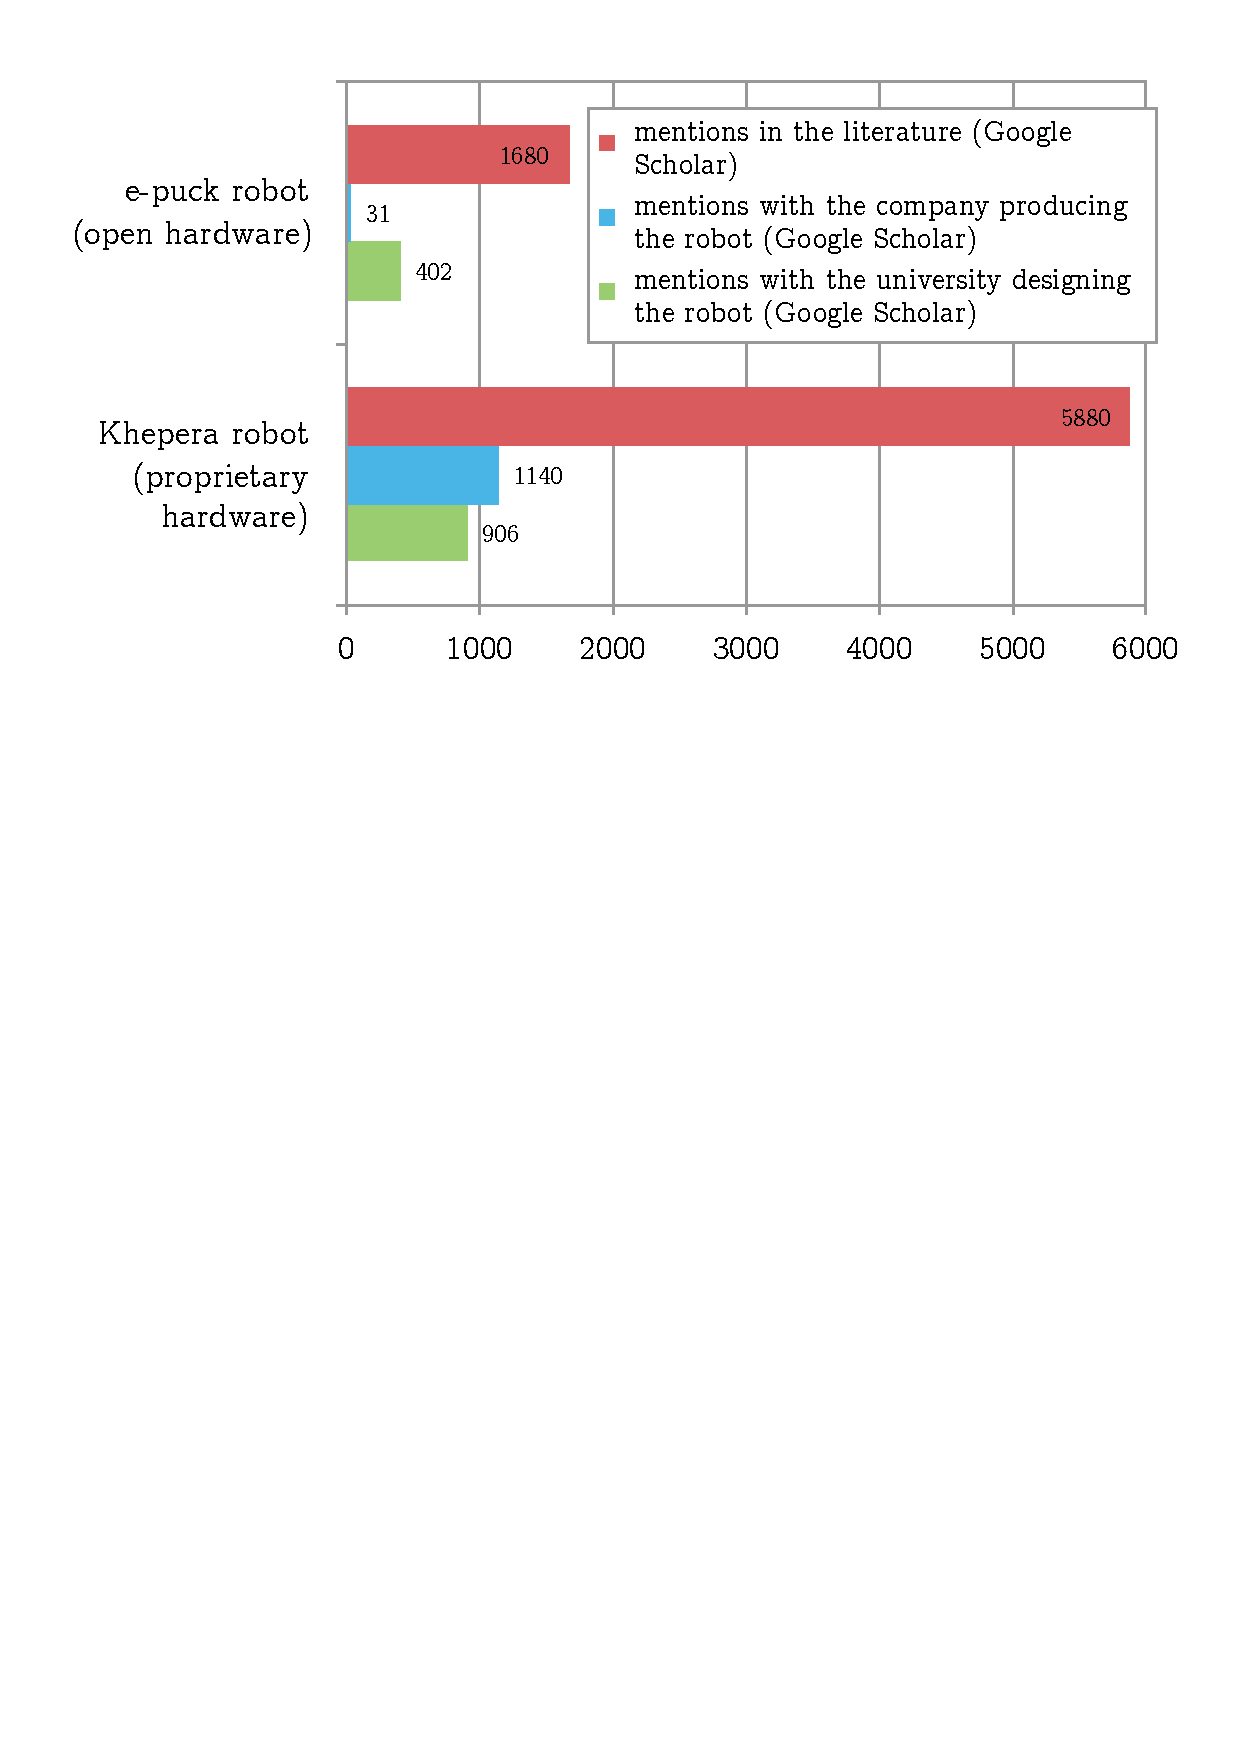
\includegraphics[width=\columnwidth]{figures/others_robots}
\caption{Comparison between e-Puck and Khepera in terms of mentions in Google Scholar, either associated with the university or with the company producing them.
%NOTE: SM: this is an analysis and should not be in caption
%between mentions in the literature, mention of the manufacturer and citation of the reference paper for two robots disseminated by our lab in the past.
%It appears that the Khepera robot, distributed with a proprietary strategy, was more linked to the company producing it than the original designers. This is the opposite for the e-puck robot, distributed with an open source license.
}
\label{fig:khepuck}
\end{figure}

Along with the institutional motivation, each contributor has a personal motivation.
%Beside the institutional motivation, there is the personal motivation of each contributor.
%The personal motivation to participate to such a project is very different than the institutional one. 
When asked about their personal motivation, the people participating in the survey cited links to their professional activity and to the specific project.
%, followed by a more general motivation by the nature of the project and finally by the engineering practice (Fig.~\ref{fig:motivation}). 
A few mentioned a more abstract goal like improving our society.
\iffalse
\begin{figure}
\centering
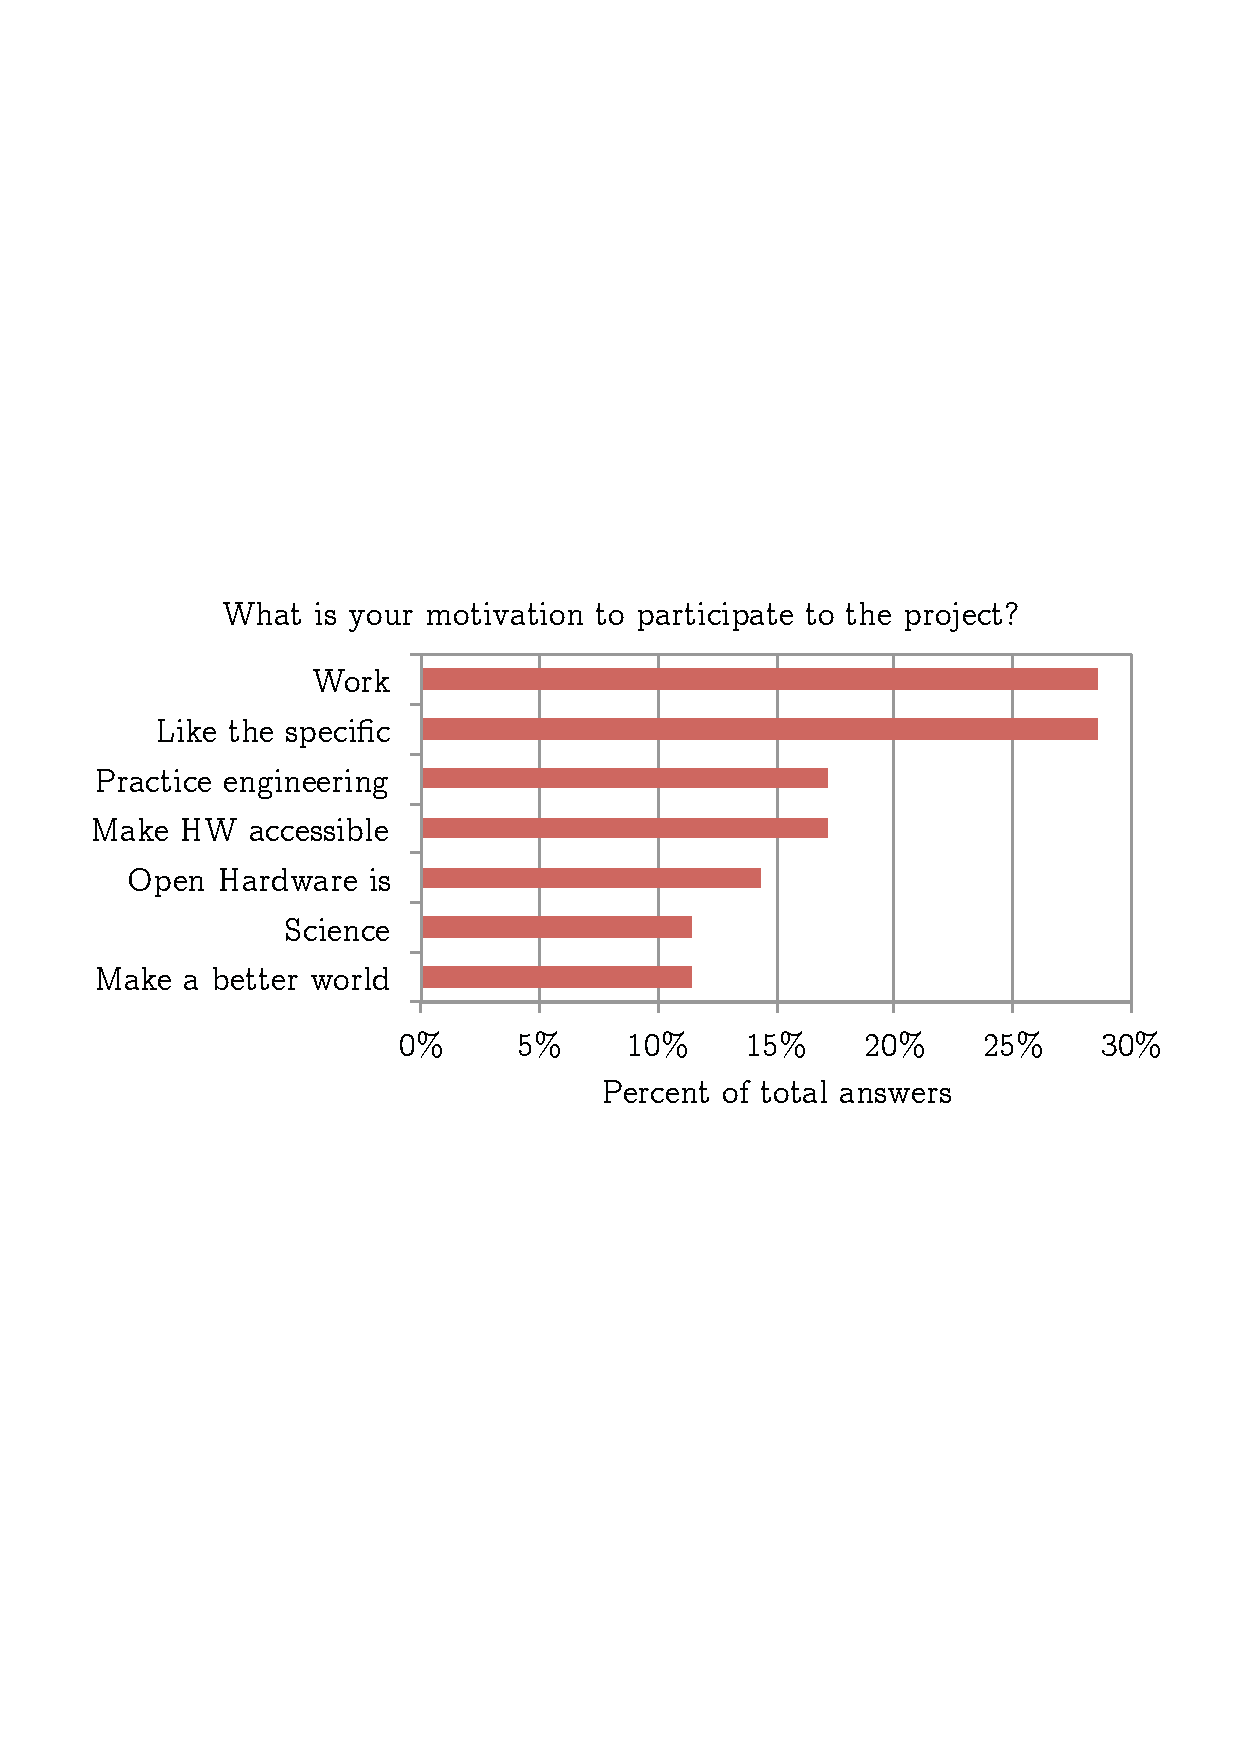
\includegraphics[width=\columnwidth]{figures/motivation}
\caption{Motivation of contributing to open source hardware.}
\label{fig:motivation}
\end{figure}
\fi

While most contributors participated in the Thymio project as part of their job, they showed a strong motivation to contribute to society, as developing a robot targeting education has an important societal component.
%were professionally involved in the professionals involved in the development of the robot because XXXX
%Industrial designers also contributed as part of an institutional project.
%Therefore the link with the professional activity and the particular project is evident.
%On another side, the motivation of contributing to society is strong in our team, as developing a robot targeting education has an important societal component.
Moreover, our project also has a strong scientific motivation; several studies are ongoing concerning the program's acceptance by teachers and the effect on children's learning.
Sharing a strong fundamental motivation, such as education or scientific achievements, is a key element for building a solid community~\cite{Stahlbrost2011}, especially if it is interdisciplinary like ours.

What benefits do people expect from participating in such a project? 
Fig.~\ref{fig:getout} shows the answers from our survey.
We can observe both a technological and a human-relations component, resulting from the community created around the project. 
%People expect to work with other people to achieve more together, to create a network, and to learn through new experience and contacts. 
Developers of the Thymio project had similar expectations.
%In the Thymio project we had similar expectations. 
Working together with several partners was for everybody a win-win situation, and creating a community of users was the only solution that allowed the development of high quality accessories and educational material.
We established a wiki\footnote{http://www.thymio.org} as the meeting point for the learners, the robot developers, and the teachers.
%This wiki introduces the robot, explains the basic behaviors, gives access to the programming environment and its documentation, and provides code samples and examples of constructions.
It is open for editing by anyone, and although we initially provided most of the material, other members of the community have started to contribute.
One of the important contributions from people outside the core design team was the translation of the wiki into four languages.

A last important motivation for having an open hardware project was because of the resulting image: we wanted a match between the non-profit nature of the project and the non-profit nature of education in general. 

\begin{figure}
\centering
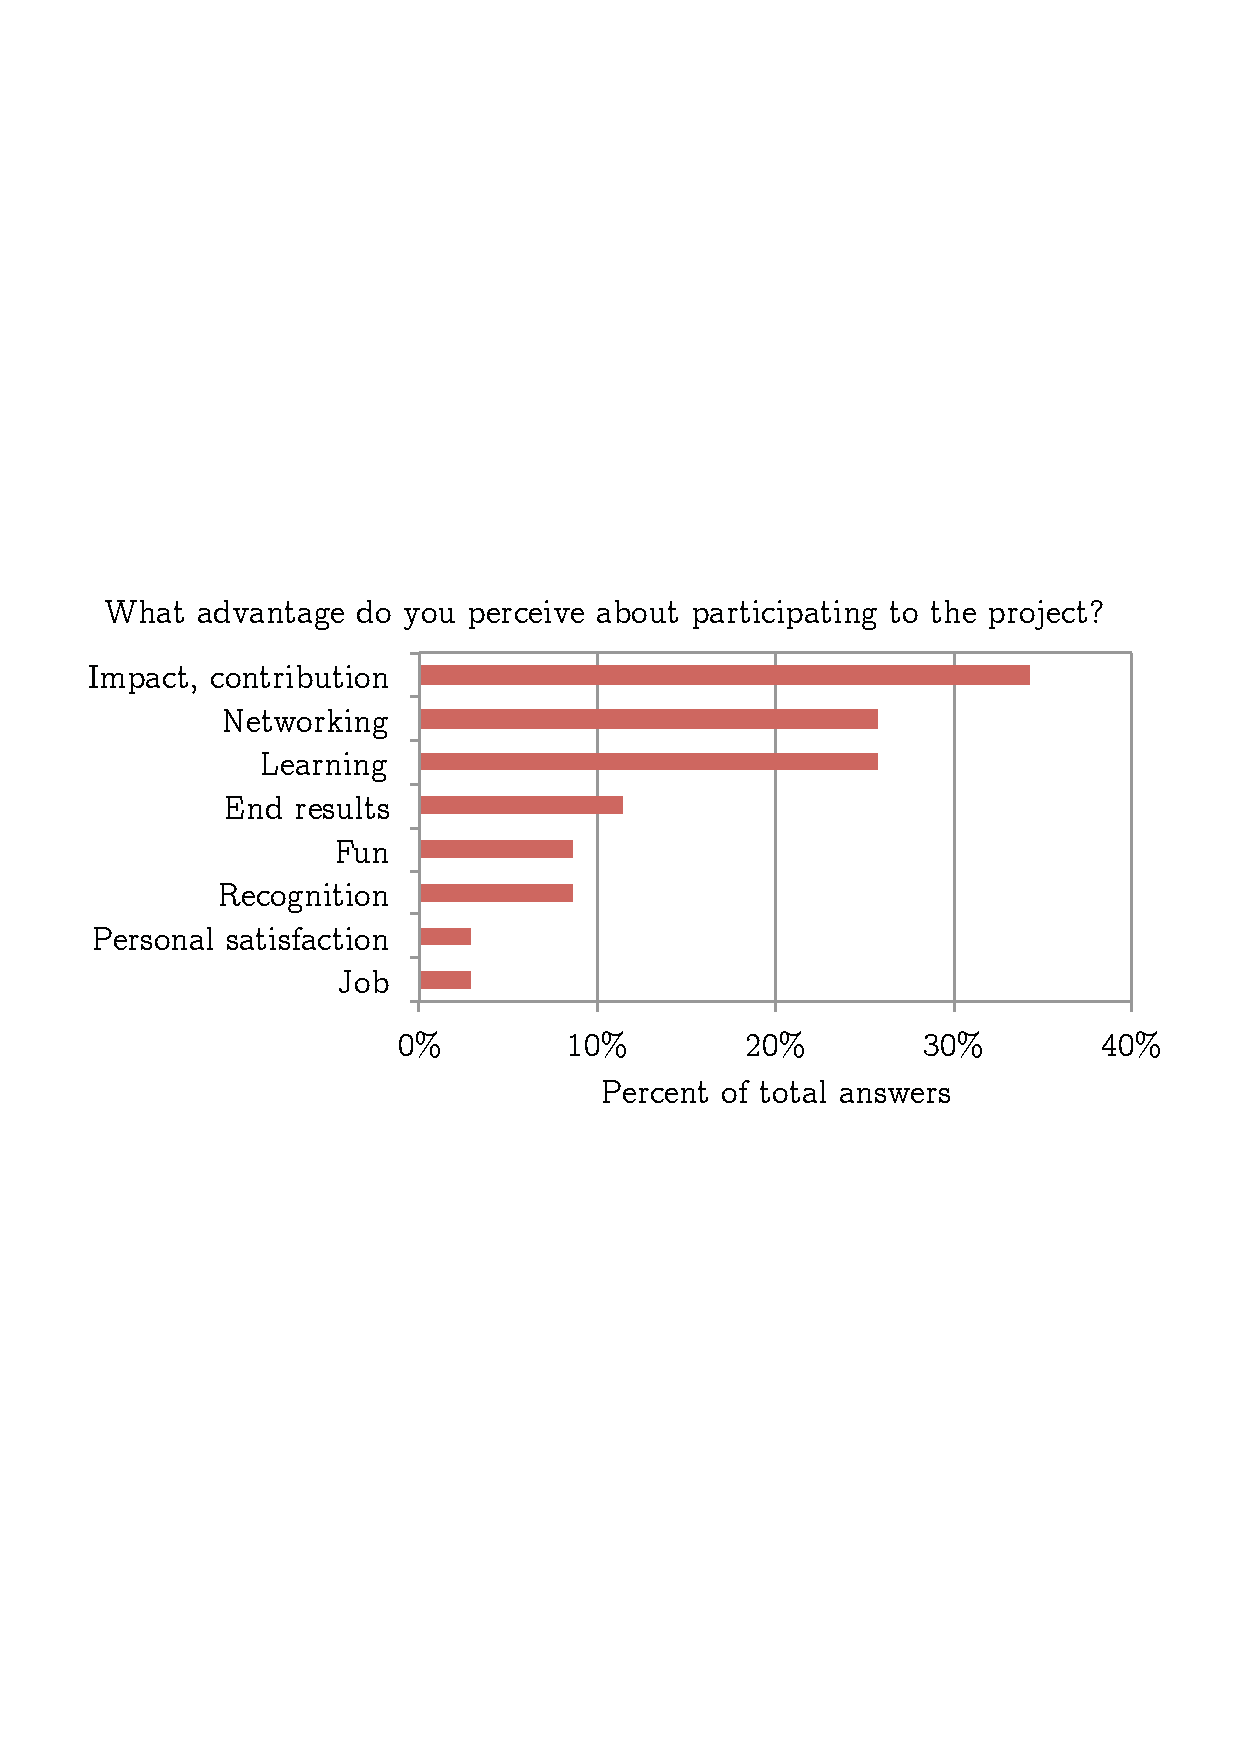
\includegraphics[width=\columnwidth]{figures/advantages}
\caption{Advantages of contributing to open source hardware.}
\label{fig:getout}
\end{figure}

\subsection{License of Project and License of Tools}

When starting an open source hardware project, one of the typical questions is which license to use when disseminating the project source files. 
All Thymio documentation and plans are distributed under the CC-BY-SA 3.0 license and the software is distributed under the LGPL license.
We will not discuss this matter here, as it is a very common and well-covered issue. 

There is another licensing issue which is less well known and that we discovered very late in our project: the constraints of the licensing of the mechanical and electronic \textsc{cad} tools. 
Indeed, when asked about this issue, 57\% of the participants in our survey were not aware of the fact that \textsc{cad} licenses can be very restrictive about the way source files can be published, and only one third checked the license on this aspect. 
%More than the half or respondents to our survey, and more than 60\% among the project leaders, state that they were not aware that this could be an issue, and only one third checked the license of their \textsc{cad} software. 
%Some stated that they did not checked the license because they were sure they can freely publish their design, but one third of them are using software not allowing the publication of source files when using educational licenses, and all these respondents are academics or students.
% FIXME: SM: there is a bit of duplication with previous sentence, I think these can be compressed
This issue is very serious, as most contributors to open source hardware projects are academics and use educational licenses that do not allow commercial use of the resulting designs. 
As producing or selling the product is part of the definition of open hardware, these licenses simply forbid publication under the standard open source hardware conditions. 

\iffalse
\begin{figure}
\centering
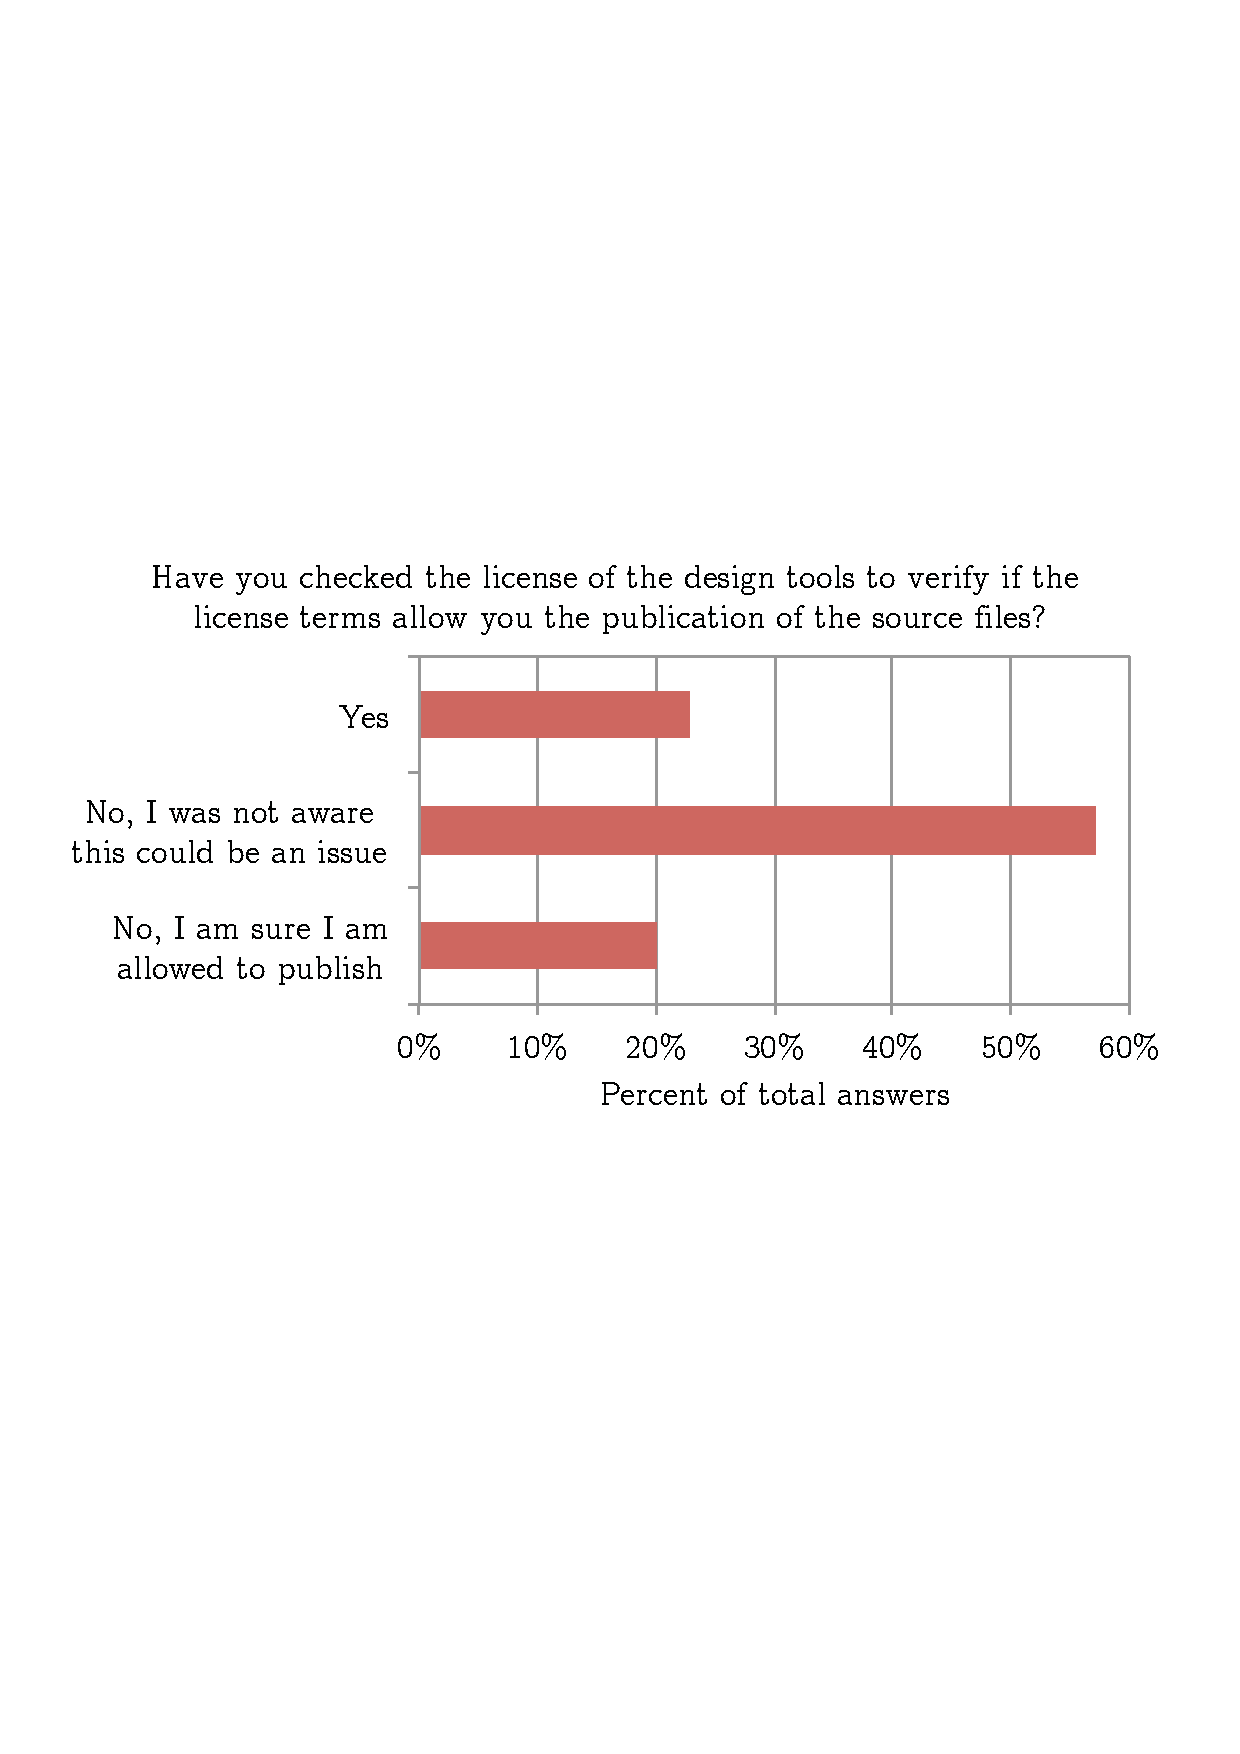
\includegraphics[width=\columnwidth]{figures/checklicense}
\caption{Awareness about \textsc{cad} tool licenses limitations.}
\label{fig:aware}
\end{figure}
\fi
To clarify this issue we contacted twelve of the major editors of mechanical \textsc{cad} and \textsc{pcb} routing software.
We asked them if their educational license allows the publication of the source files. %, and we specified that the published files could have been downloaded by a company to produce the system for commercial purposes.
Fig.~\ref{fig:editors} summarizes the results of this survey.
Only three of the twelve editors have education licenses allowing this type of publication. 
Two others explicitly mentioned the possibility if permission were requested before publication.
A large mechanical \textsc{cad} editor was puzzled by our questions and after realizing the impact of the license, introduced a special condition allowing publication of files in clearly labeled open source hardware projects.
In previous situations concerning open source publication, the same editor asked the universities to purchase commercial licenses to permit publication.
This can multiply by factors of hundreds the price of the \textsc{cad} license.
%This blocking factor for open hardware also applies to the publication of scientific results, as promoted by many governments in the last decade and generally called ``open science''.
%The change of policy in \textsc{cad} files publication that we obtained is a sign of the very positive trend set by open hardware and by open science in general.

\begin{figure}
\centering
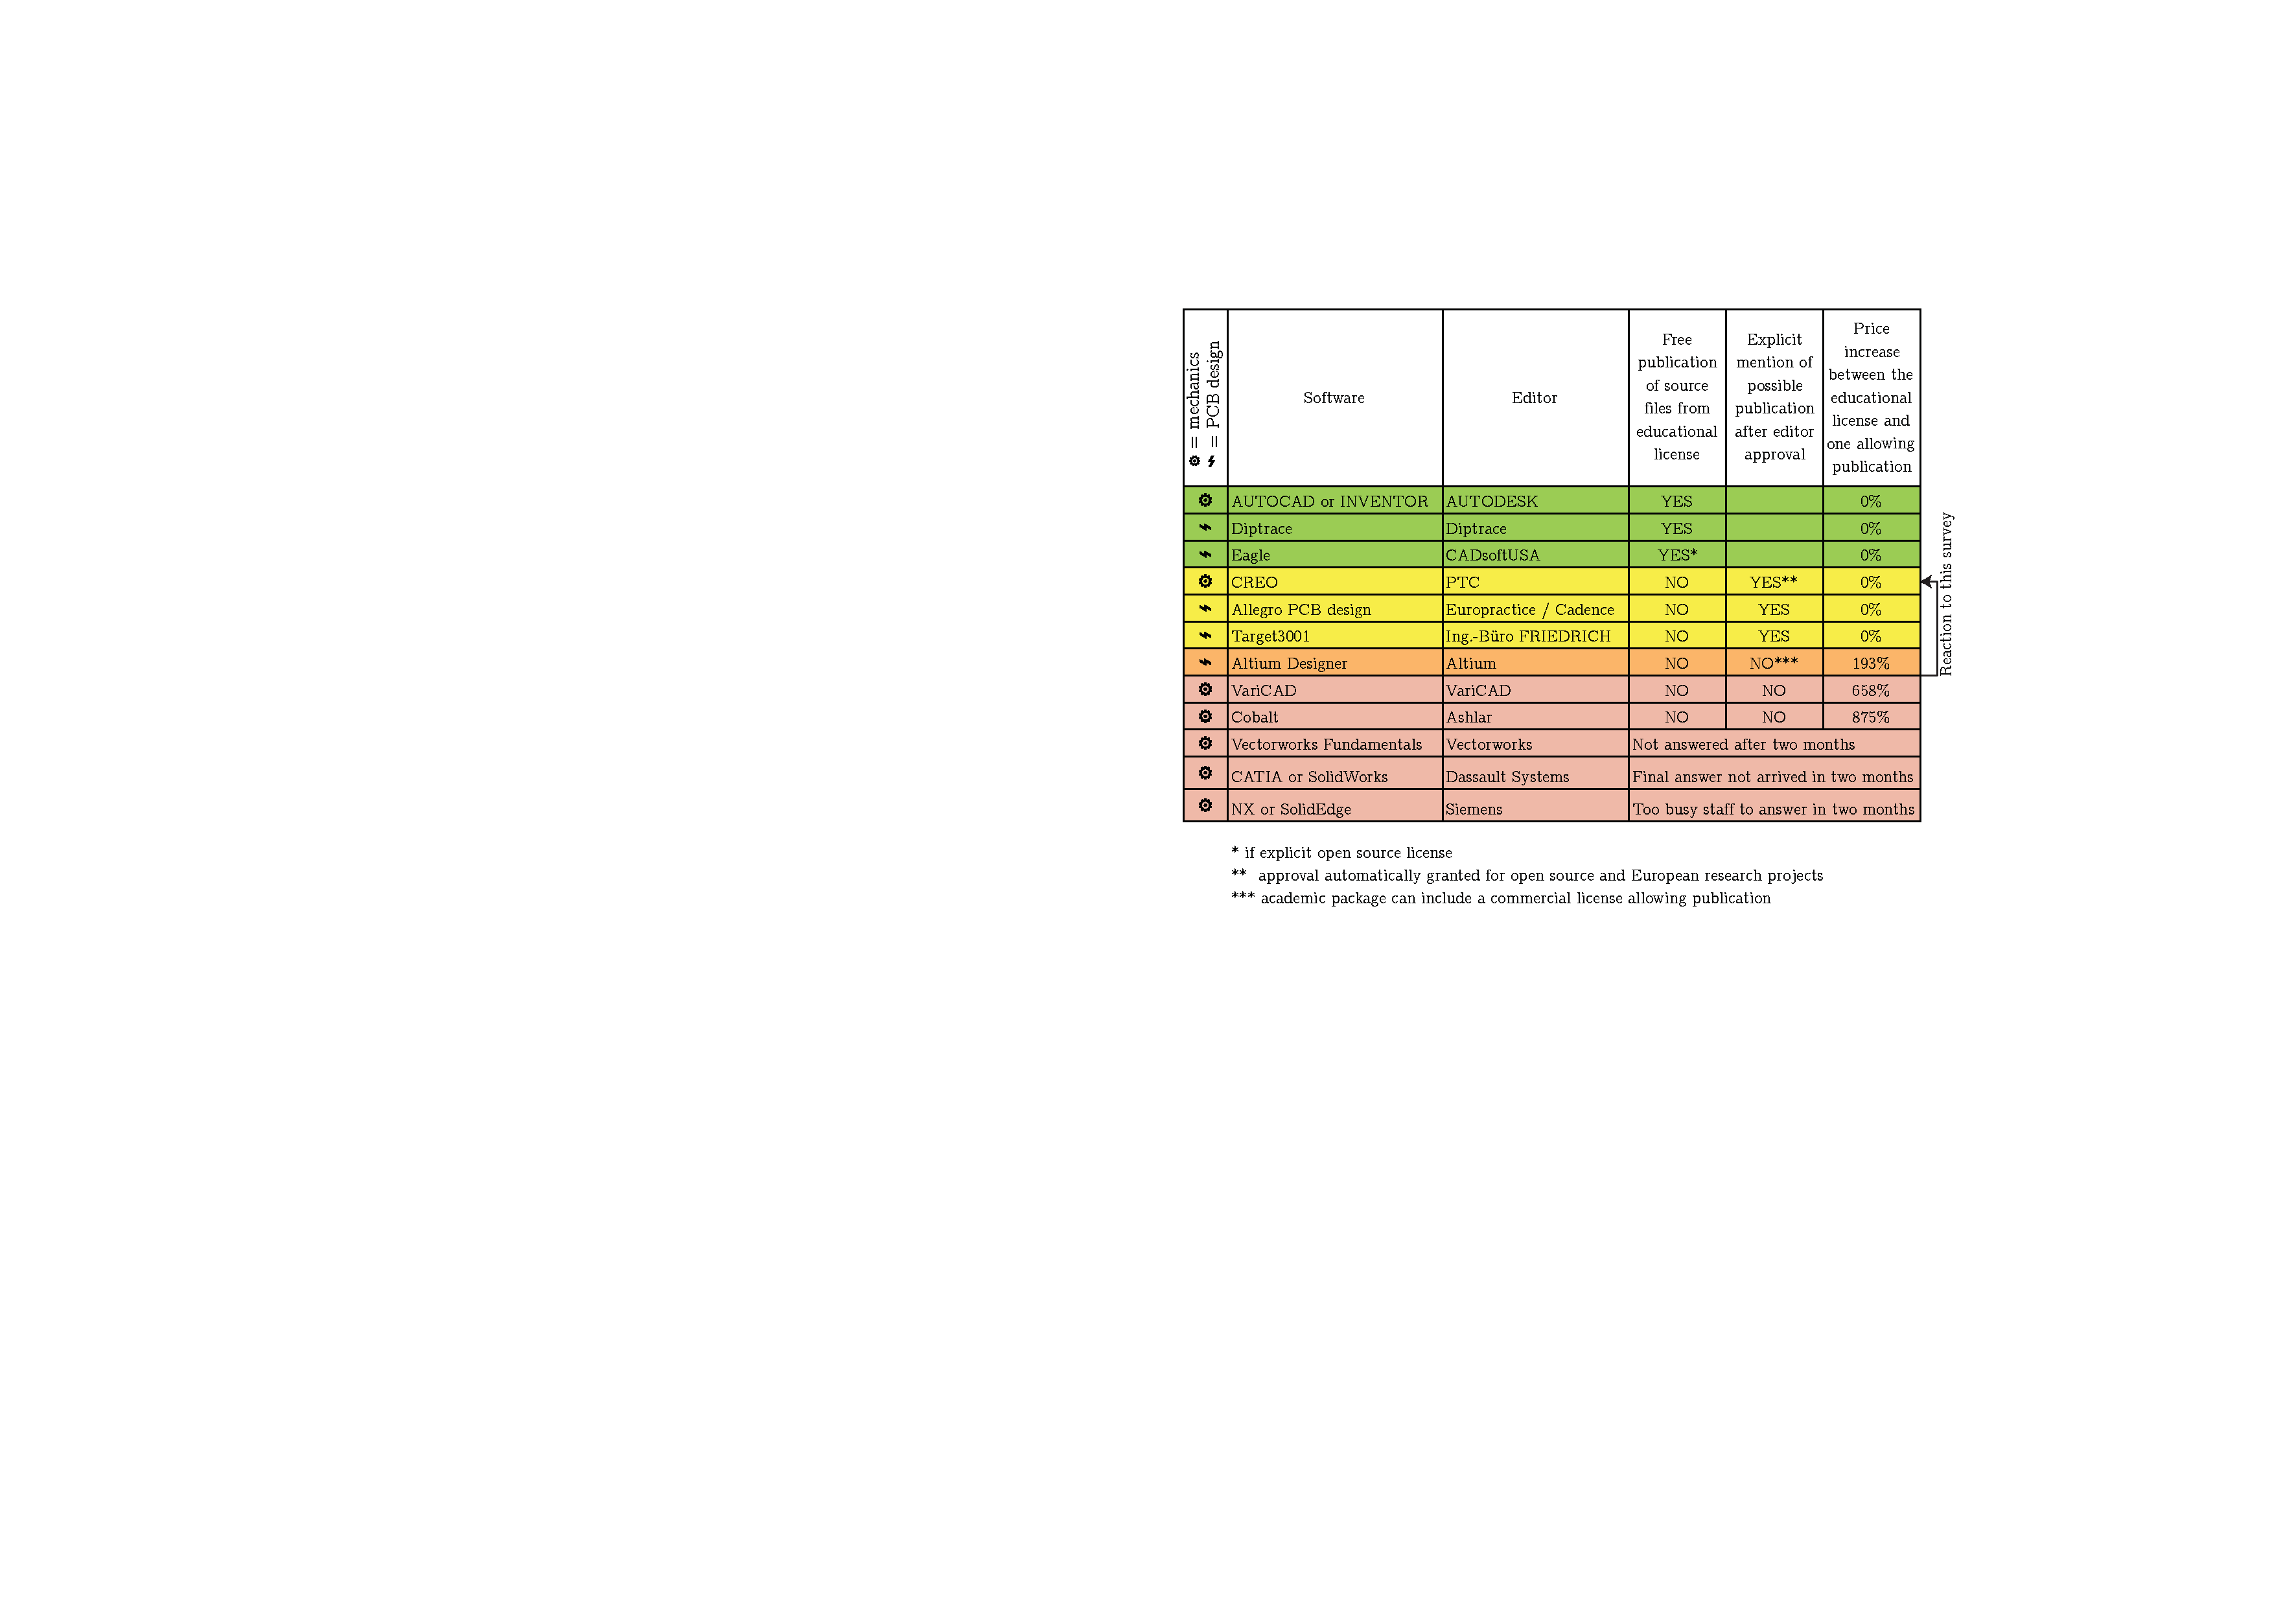
\includegraphics[width=\columnwidth]{figures/table}
\caption{Publication possibilities as function of the \textsc{cad} editors, as of the end of March 2016.}
\label{fig:editors}
\end{figure}

This legal issue is totally underestimated by both people participating in such projects and by the \textsc{cad} editors, and it is a potential threat for many projects. 
%In a period where editors are looking for additional revenues and are attacking universities for misuse of licenses\footnote{We are aware, just in Switzerland, of two situations where large amounts of money are asked to universities for non-respect of software licenses.}, this can be a very dangerous situation.

\subsection{Who Designs, Produces, and Supports the Hardware}

%Among the fundamental choices when starting an open source hardware project, there is the choice of the type of production. 
In the definition of open hardware given at the beginning of this paper, it is stated that one should offer ``hardware whose design is made publicly available so that anyone can [\dots] make [\dots] hardware.''
Should ``anyone'' mean every single person or only companies able to produce the product?
%This choice has implications on who designs the system and how.

In our project, we decided to have two different types of hardware: the robot itself and the accessories. % used in specific activities.
The robot is the expensive part and has a very neutral design, allowing adaptation to specific situations.
This adaptation is achieved by custom accessories that increase the attractiveness of the robot in its specific role, enabling activities for different ages and genders.

For the robot itself, we opted to interpret ``anyone'' as only the professional structures able to mass-produce hardware based on the price and complexity of the product. 
%When looking for the best performance per price ratio, we decided to use techniques that require heavy equipment.
%For instance we decided to produce all mechanical parts by injection molds. 
%This ensures a price per part of some cents, which cannot be achieved by others techniques.
%Letting end-user produce their own parts would results in higher prices for less performances. 
%This choice has another implication: only a core team of highly skilled engineers can contribute to the project. 
%It is not trivial to design a mechanical part that can be molded in the simplest possible way.

For the accessories, less technically challenging and stronger linked with creativity and educational value, we promoted techniques that are accessible to ``anyone'' in the broader sense: paper, cardboard, LEGO\textsuperscript{\textregistered} constructions and 3D printing. %, as explained in section~\ref{sec:crea} and illustrated in Fig.~\ref{fig:example-construction}.
This allows a much broader spectrum of contributors, including teachers and lay people.

\iffalse
\begin{figure}
\centering
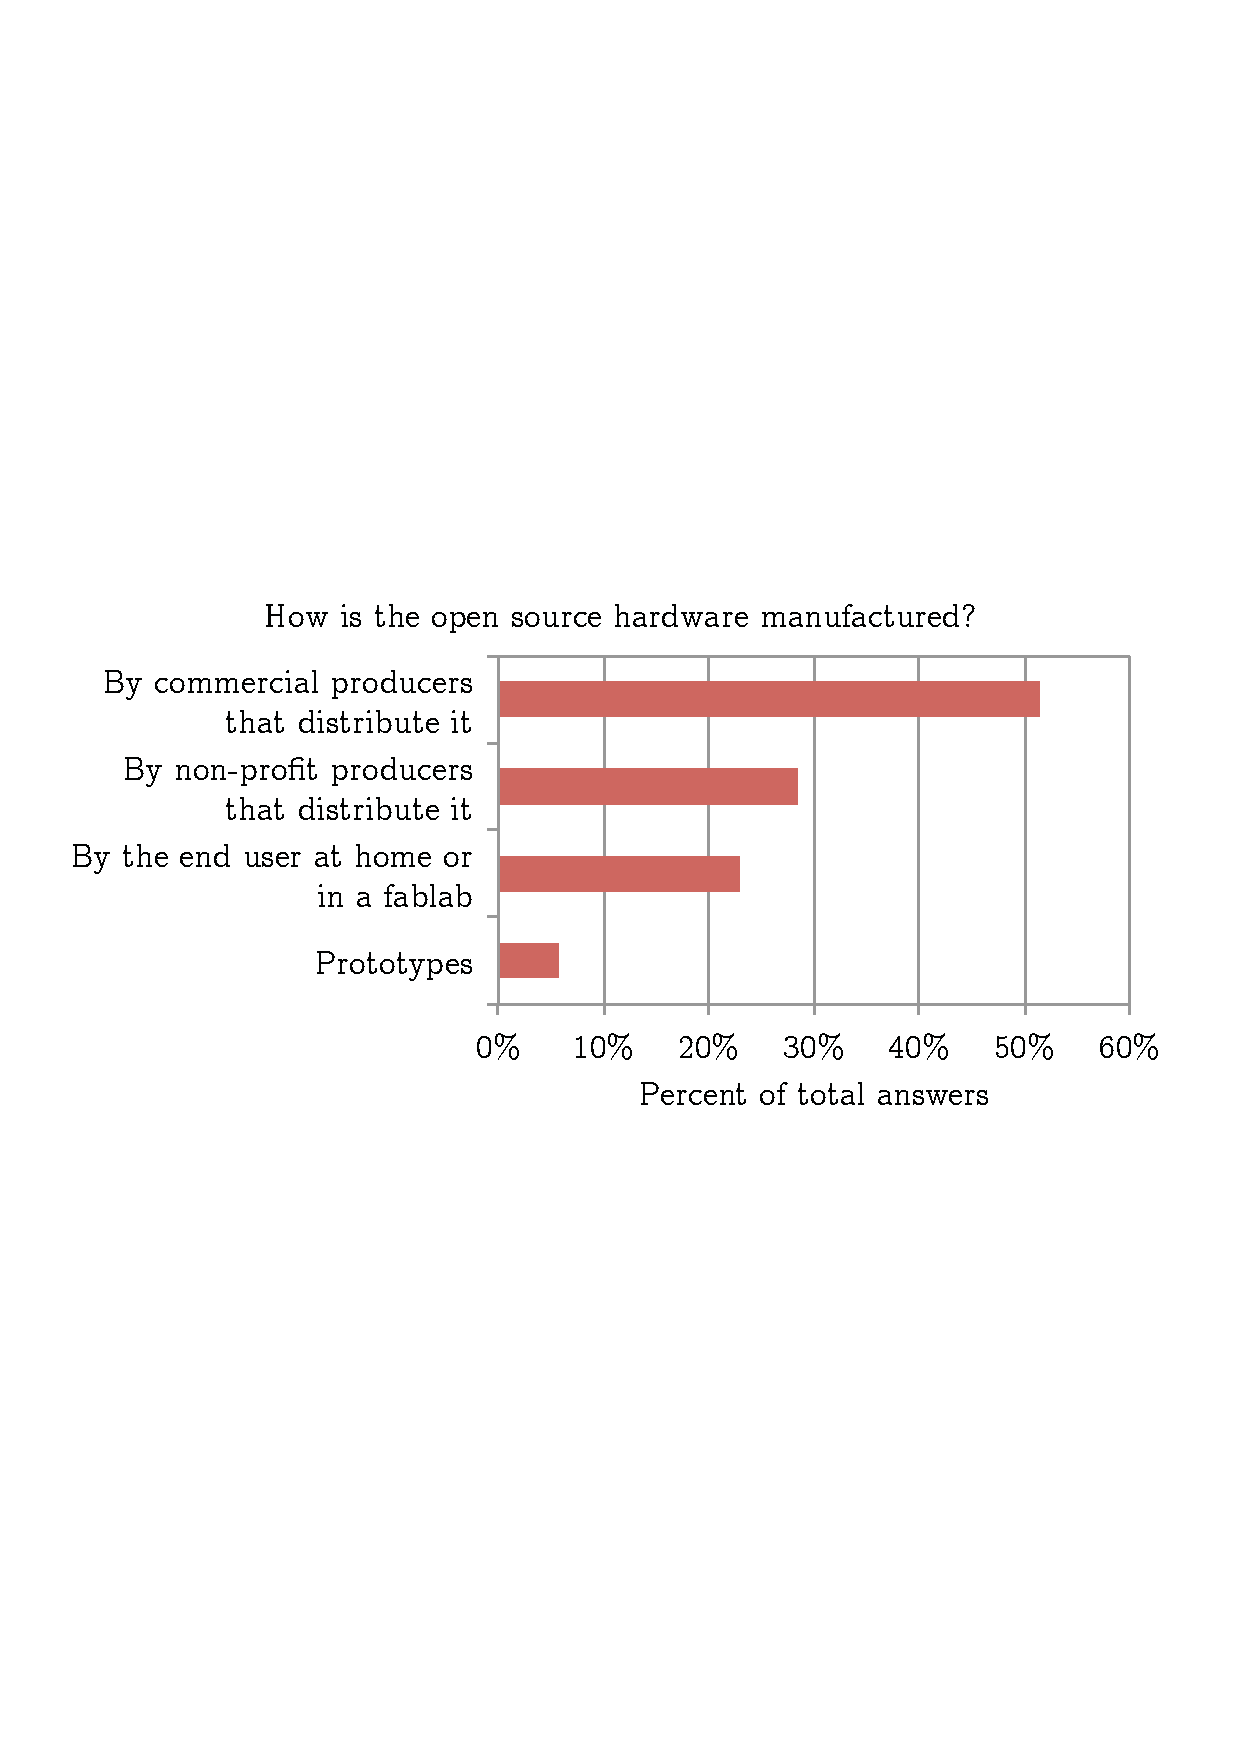
\includegraphics[width=\columnwidth]{figures/manufacturing}
\caption{Production methods in the mentioned projects.}
\label{fig:production}
\end{figure}
\fi

%Our survey shows that the most common production method is a centralized one by commercial companies.% (Fig.~\ref{fig:production}).
%Indeed, large open source hardware projects like Arduino are based on this model.
%One could argue that this model makes these robotic projects close to standard commercial models, leading to a lack of involvement from users and loosing the open source spirit.
%In our case, we decided to alleviate this effect by creating a non-profit association, called Mobsya, in charge of producing and selling the robots. 
%While anybody else could produce the Thymio follwing a more buiness-oriented model, the initial production has been done respecting a coherent and global non-profit strategy, in line with educational values of the community of users.
%Moreover, the users are better integrated in the second layer of open source hardware consisting of accessories, where anybody can contribute their own designs and put them on the wiki.

%Another strong difference between a standard consumer product and our vision of open hardware is that Thymio should be durable.
Another strong element of our vision of open hardware is that Thymio should be durable.
%Schools do not have large budgets for technological tools and make strong investment in training of their teachers when adopting a new tool.
As schools invest in long term training of teachers, for instance, the lifetime of the products should also be as long as possible. 
The open hardware approach fits well to this requirement, as it gives to the user, or to a generic technician, better conditions to repair the system, having the specifications of all components. This is not the case of commercial robots like Edison, for instance.
Supporting this type of operation has an impact on the robot design; for instance Thymio can be easily opened with four standard screws, and we introduced connectors between key elements such as motors, speaker, the battery and the main \textsc{pcb}.
Another key element in supporting repairs by end users is the documentation of calibration methods. 
When choosing very low cost components, one faces large dispersion of characteristics. 
For example, in the Thymio the right and left wheel motors can differ in their electrical characteristics, resulting in the robot not going straight for similar speed commands to both wheels.
To correct this problem, we introduced factory calibration. %, storing in the microcontroller memory correction factors that are specific for each robot. 
To allow the user to replace a broken motor, it is essential to give him also the possibility to re-calibrate the robot and adjust the parameters of the new motor.
In Thymio, this results in the design and the documentation of calibration processes that can be performed by anyone, getting close to the original definition of open source hardware.

\iffalse
\subsection{Added value of open source hardware in distribution}

Beside the sale of more than 10'000 robots by Mobsya, there are several elements that show a specific advantage of having chosen an open source hardware model.

The first element is linked to the financial support of the project.
Although the non-profit nature of the project blocked the possibility of having shareholders injecting capital, this same nature enabled a lot of institutional donations linked with the societal goal of the project.
The financial support through donations instead of acquisition of shares, allows keeping a total decisional freedom and void debts at the same time.
The main disadvantage of this approach is the amount of financial support, limited in our case to several hundreds of thousands of dollars. 

The second interesting element of the open source hardware approach is the very high acceptance of the resulting robot by universities and their offices in charge of promotion of science.
Although these are not the primary users targeted by the robot, these are institutions with high visibility and influence on school programs. 
In particular INRIA in France and the University of Cambridge in the United Kingdoms decided to use Thymio as tool for promoting their activities and introduced it into schools.
In France, INRIA developed several teaching modules and supported the training of more than 1000 teachers to the use of Thymio. 
This resulted in Thymio being one of the tools chosen for the education of digital science in the reference books of the French Academy of Science and its foundation for promotion of science in education, called ``La main \`a la p\^ate.''
The open source nature of Thymio gives these institutions a large control, as they can ensure maintenance and even further develop the robot.
The impulsion given by the academic institutions has been followed by many teachers who contributed their own teaching material. 
Currently one can find more than 50 teaching modules, a large tutorial, and many reports on school activities using Thymio. 

In some cases, the open source nature of this project was a crucial political argument for the choice of this platform.
For instance, in Geneva, Switzerland, the state government decided to move toward open source non-proprietary tools in education.
All primary school and most secondary school computers have been installed with the Ubuntu distribution of Linux. 
On this operating system the LEGO\textsuperscript{\textregistered} Mindstorms\textsuperscript{\textregistered} software tools are not available, and their proprietary nature is not compatible with the philosophy dictated by the government. 
Thymio was therefore extremely welcome, and the state of Geneva organized their own training courses for teachers, adapted existing educational materials to their own curriculum and organized a lending system for all schools that cannot afford to buy the robots.

% FIXME: SM: in case of space limit, I would remove the following paragraph
%Finally, the non-profit nature of the project, including the production infrastructure, has contributed to reduce the obstacle toward the acquisition of this platform for many schools, where teachers have a strong societal motivation and are reluctant to use tax-payers money to pay the divident of some shareholders.

\subsection{Problems of open-source hardware projects}

\begin{figure}
\centering
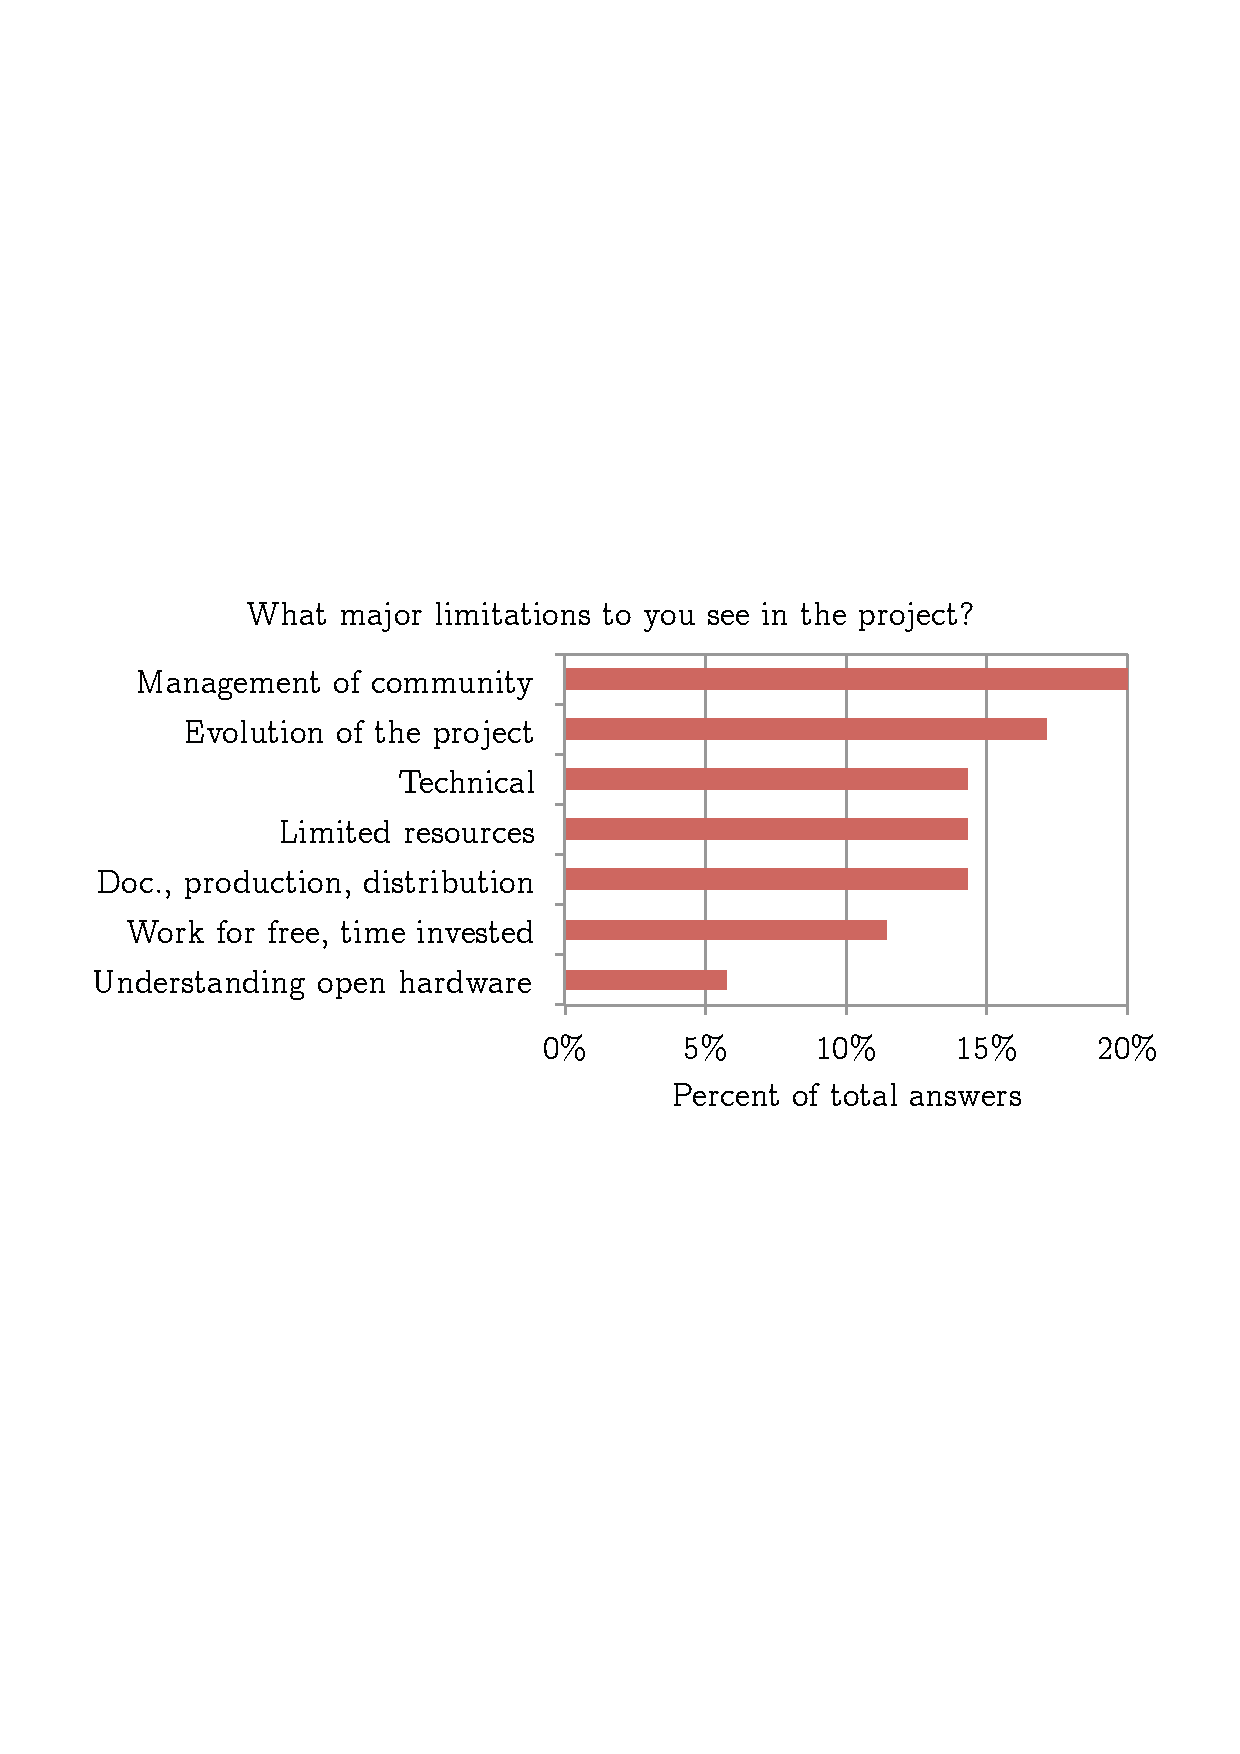
\includegraphics[width=\columnwidth]{figures/limitations}
\caption{Limitations of open source hardware projects.}
\label{fig:problems}
\end{figure}

The very specific structure of an open-source hardware project has also drawbacks. 
Asked about problems met in their project (Fig.~\ref{fig:problems}), the participants to our survey mention the management of the community, the evolution of the project, the efforts in documentation, production and distribution and the limited resources.
These problems are mainly caused by the mismatch between the conditions of the initial phase of the project, and the needs of long term sustainability.
Initially, these projects are created by academic people with engineering background, typically in a flat structure.
However, long term sustainability requirements are closer to the ones of a successful startup, and involve communication, marketing, and professional management in order to acquire sustained funding.
Yet, 62\% of the participants to our survey report projects that are managed by the founder of the initiative, who might not be the best person to lead such a structure.
This differs from open-source software, because in our model initiating hardware production requires the investment of a large amount of money, and modifying hardware is much slower than modifying software.
Moreover, in the case of robotics, although software plays a critical part, the perception of the product is highly centered on the hardware, creating tensions between hardware- and software-oriented people.
Therefore, to grow such open hardware projects, there is a structural conflict between open-source ideals (for example meritocratic decision process) and the concrete financial and logistic constraints.

% There are here two kinds of problems: one of management of people, the other in the development of the project after the first design.
% The management of the project seems a recurrent problem and is related to the nature of this type of structure, mainly very flat and built on academic people with engineering background. 
% More than 62\% of the answers to our survey report about projects that are managed by the founder of the initiative and not by the most expert in the field or by a manager, which is perhaps not the best objective choice.
% It is indeed very difficult to evolve from a phase where the engineering is the core of the project, to a new phase where communication and management play an increasing role.
% This problem is deeply connected with the one of acquiring sustained funding for the project, in order to build a professional team able to support the product.
% The same holds for several other factors, like the efforts in documentation, production and distribution of the product. 
% Also here there is a change of activity from the very creative and appealing design phase, to a phase of documentation and, in some cases, production and distribution which is not at all the same type of activity and requires different skills.
% This shift requires extra efforts and motivation, which are often missing, especially for activities like documentation that are not appreciated by engineers.
% In general many respondents to our survey identified the evolution of the project as a general problematic issue, which summarizes the several aspects mentioned above.

In the Thymio project we have addressed these problems by having several partners, each of them specialized in one aspect: design, production and sale, creation of educational material, etc.
Despite this approach, we also encountered difficulties in nurturing an active community covering all aspects of the project, and issues in finding a long term vision that both injects life into the project and is financially sustainable.
This is especially difficult with a large number of partners, as differing views can result in conflicts. 
A key element that allowed to keep cohesion in our community was to share, among all partners, strong basic values about improvement of society through education.
\fi


\section{Conclusion}

%XXXXX present a better overview of the significant improvements that the design choices bring in relation to the design goals  XXXXXXX
The introduction of robots in formal education is a very challenging task, not only because of technical requirements such as low cost and interactivity, but also because of factors depending on the school environment, such as the diversity of the educational programs, the dependence on local structures and languages, or the required training of teachers.
Most of the current educational robotic activities capitalize upon one strong element, for instance the technical innovation, but miss to match the formal education requirements.
%Because they do not consider all elements at stake, these tools fail to meet some challenges of formal education.
%On the contrary, in this paper we presented a global approach that tackles these questions in a holistic way, based on open source and non-profit principles.
%The result is the Thymio robot and its surrounding open source community including engineers, art designers, production and sales people, and teachers.
%The open source hardware and the related contributions are split in two categories: the robot itself, produced by a non-profit organization and requiring very advanced skills in both design and production, and the accessories for activities, based on techniques broadly accessible and with a larger panel of contributors.

The open source hardware approach used in the Thymio project addresses this and several other issues found in educational robotics.
The inclusion of education scientists, teachers and designers is possible because of the open nature of the project and the split between core technology, produced in a central way, and accessories, accessible with DIY approaches. This split allowed to ensure also a gender- and age-neutral basic robot.
This large inclusion of users and contributors allowed the production, in parallel to the robot technology, of a large set of pedagogic scenarios.

The philosophy of open source and free access to information fits extremely well with the community of users in education, and was reinforced by producing the robot in a non-profit structure.
This approach allowed to broadly distribute the robot with minimal changes dues to management of intellectual properties, royalties, financial support and so on.
Moreover, the open source approach allows to provide a durable robot, easy to maintain and repair, with at the same time a community of users providing educational material and mutual support.

By making a survey among contributors to open source hardware projects, we could observe that our project shares some characteristics with the majority of the projects represented in the survey. 
%We also faced difficulties in establishing the community, we chose production and distribution methods that are broadly applied, and we share most of the motivational elements that are behind other projects.
We identified for instance an underestimated legal issue for open source hardware projects in the licensing term of \textsc{cad} software.
%Indeed only very few editors have licenses allowing the publication of source files created with educational license.
%Two surveys among the users and the \textsc{cad} editors show that both people contributing or leading open source hardware projects and the editors themselves are not aware of this issue.
Finally, we could show some elements, specific to educational robotics, that differentiate our project from other open source hardware projects.
In particular, our project takes advantage of an alignment between the principles underlying open source and the nature of education institutions. 
%This fits a political trend toward open source in education and in science in general.
We also found a solution to the problem of production methods by splitting our hardware in two categories, enabling both advanced technology for the robot and a large variety of accessories.
Hence, Thymio appeals to a broad community of end users in education, addressing durability and inclusion at several levels.

\bibliography{ThymioEdu}
\bibliographystyle{ieeetr}

%-\addtolength{\textheight}{-12cm}   % This command serves to balance the column lengths
                                  % on the last page of the document manually. It shortens
                                  % the textheight of the last page by a suitable amount.
                                  % This command does not take effect until the next page
                                  % so it should come on the page before the last. Make
                                  % sure that you do not shorten the textheight too much.

%%%%%%%%%%%%%%%%%%%%%%%%%%%%%%%%%%%%%%%%%%%%%%%%%%%%%%%%%%%%%%%%%%%%%%%%%%%%%%%%



%%%%%%%%%%%%%%%%%%%%%%%%%%%%%%%%%%%%%%%%%%%%%%%%%%%%%%%%%%%%%%%%%%%%%%%%%%%%%%%%



%%%%%%%%%%%%%%%%%%%%%%%%%%%%%%%%%%%%%%%%%%%%%%%%%%%%%%%%%%%%%%%%%%%%%%%%%%%%%%%%
%\section*{APPENDIX}
%
%questionnaire?
%
%\section*{ACKNOW\textsc{led}GMENT}
%
%??



%%%%%%%%%%%%%%%%%%%%%%%%%%%%%%%%%%%%%%%%%%%%%%%%%%%%%%%%%%%%%%%%%%%%%%%%%%%%%%%%


\end{document}
